\documentclass[11pt,a4paper,openany]{book}

% --- Typography and page geometry -------------------------------------------------
\usepackage[margin=28mm,inner=31mm,outer=25mm,headheight=16pt,footskip=16mm]{geometry}
\usepackage{fontspec}
\usepackage{mathtools}
\usepackage{unicode-math}
\IfFontExistsTF{EB Garamond}
  {\setmainfont{EB Garamond}}
  {\setmainfont{Latin Modern Roman}}
\IfFontExistsTF{Noto Sans}
  {\setsansfont{Noto Sans}[Scale=0.90]}
  {\setsansfont{DejaVu Sans}[Scale=0.90]}
\setmonofont{DejaVu Sans Mono}[Scale=0.82]
\IfFontExistsTF{Asana Math}
  {\setmathfont{Asana Math}}
  {\setmathfont{Latin Modern Math}}
\usepackage{microtype}
\usepackage{setspace}
\setstretch{1.045}

% --- Structure, tables, code, diagrams -------------------------------------------
\usepackage{xcolor}
\usepackage{graphicx}
\usepackage{booktabs}
\usepackage{tabularx}
\usepackage{longtable}
\usepackage{array}
\usepackage{enumitem}
\usepackage{titlesec}
\usepackage{fancyhdr}
\usepackage{fvextra}
\usepackage[most]{tcolorbox}
\usepackage{tikz}
\usepackage{xurl}
\usetikzlibrary{arrows.meta,positioning,fit,calc,shapes.geometric,backgrounds}
\usepackage{hyperref}
\usepackage{bookmark}
\usepackage[nameinlink,noabbrev]{cleveref}

% --- Palette ----------------------------------------------------------------------
\definecolor{Ink}{HTML}{24302B}
\definecolor{Olive}{HTML}{68745A}
\definecolor{OliveDark}{HTML}{46523D}
\definecolor{Sage}{HTML}{E8ECE1}
\definecolor{Warm}{HTML}{F5F1E7}
\definecolor{Sand}{HTML}{DED4BE}
\definecolor{BlueGray}{HTML}{50656B}
\definecolor{Coral}{HTML}{A65F52}
\definecolor{CodeBg}{HTML}{F6F7F3}
\definecolor{RuleGray}{HTML}{AAB1AC}

\pdfstringdefDisableCommands{
  \def\module#1{#1.lean}
  \def\decl#1{#1}
  \def\code#1{#1}
  \def\upfun{up}
  \def\Fabius{F}
  \def\TM{tm}
  \def\R{R}
  \def\Q{Q}
  \def\N{N}
  \def\Z{Z}
  \def\C{C}
}

\hypersetup{
  colorlinks=true,
  linkcolor=OliveDark,
  citecolor=BlueGray,
  urlcolor=Coral,
  pdfauthor={OpenAI, prepared for Vladimir Reshetnikov},
  pdftitle={The Fabius Function in Lean: A Source-Level Walkthrough},
  pdfsubject={Architecture, dependencies, and proof ideas of the FabiusFunction Lean library},
  pdfkeywords={Lean 4, Fabius function, Rvachev up function, Thue-Morse, dyadic rationals, asymptotics}
}

% --- Heading and running-head design ---------------------------------------------
\titleformat{\chapter}[display]
  {\normalfont\sffamily\bfseries\color{Ink}}
  {\filleft\fontsize{42}{44}\selectfont\color{Sand}\thechapter}
  {-14pt}
  {\titlerule[0.8pt]\vspace{1.1ex}\Huge}
  [\vspace{1ex}\titlerule]
\titleformat{\section}{\Large\sffamily\bfseries\color{OliveDark}}
  {\thesection}{0.7em}{}
\titleformat{\subsection}{\large\sffamily\bfseries\color{BlueGray}}
  {\thesubsection}{0.7em}{}
\titleformat{\subsubsection}{\normalsize\sffamily\bfseries\color{Ink}}
  {\thesubsubsection}{0.7em}{}
\titlespacing*{\chapter}{0pt}{-18pt}{26pt}

\pagestyle{fancy}
\fancyhf{}
\fancyhead[LE]{\small\sffamily\color{OliveDark}\leftmark}
\fancyhead[RO]{\small\sffamily\color{OliveDark}\rightmark}
\fancyfoot[LE,RO]{\small\sffamily\color{Ink}\thepage}
\renewcommand{\headrulewidth}{0.35pt}
\renewcommand{\chaptermark}[1]{\markboth{\thechapter.\ #1}{}}
\renewcommand{\sectionmark}[1]{\markright{\thesection.\ #1}}

% --- Semantic helpers --------------------------------------------------------------
\newcommand{\R}{\ensuremath{\mathbb{R}}}
\newcommand{\Q}{\ensuremath{\mathbb{Q}}}
\newcommand{\N}{\ensuremath{\mathbb{N}}}
\newcommand{\Z}{\ensuremath{\mathbb{Z}}}
\newcommand{\C}{\ensuremath{\mathbb{C}}}
\newcommand{\Fabius}{\ensuremath{\operatorname{F}}}
\newcommand{\upfun}{\ensuremath{\operatorname{up}}}
\newcommand{\TM}{\ensuremath{\operatorname{tm}}}
\newcommand{\module}[1]{\nolinkurl{#1.lean}}
\newcommand{\decl}[1]{\texttt{\detokenize{#1}}}
\newcommand{\code}[1]{\texttt{\detokenize{#1}}}
\newcommand{\commit}{\nolinkurl{40c0d637d310a9f16d96f53d287438b7d9b1f53f}}
\newcommand{\pathbreak}[1]{\nolinkurl{#1}}
\newcommand{\sourcepath}[1]{\par\smallskip\noindent\textcolor{OliveDark}{\sffamily\bfseries Source:}\quad\pathbreak{#1}\par\smallskip}

\setlist[itemize]{leftmargin=1.45em,itemsep=0.28em,topsep=0.35em}
\setlist[enumerate]{leftmargin=1.6em,itemsep=0.30em,topsep=0.35em}
\setlist[description]{style=nextline,leftmargin=1.5em,labelindent=0pt,itemsep=0.45em,topsep=0.4em,font=\normalfont\sffamily\bfseries\color{OliveDark}}

% --- Code blocks ------------------------------------------------------------------
\DefineVerbatimEnvironment{LeanCode}{Verbatim}{
  fontsize=\small,
  frame=single,
  framesep=3mm,
  rulecolor=\color{RuleGray},
  fillcolor=\color{CodeBg},
  breaklines=true,
  breakanywhere=true,
  breaksymbolleft={},
  tabsize=2,
  baselinestretch=1.0
}
\DefineVerbatimEnvironment{ShellCode}{Verbatim}{
  fontsize=\small,
  frame=single,
  framesep=3mm,
  rulecolor=\color{RuleGray},
  fillcolor=\color{Warm},
  breaklines=true,
  breakanywhere=true,
  breaksymbolleft={},
  tabsize=2,
  baselinestretch=1.0
}

% --- Callouts ---------------------------------------------------------------------
\newtcolorbox{proofidea}[1][]{
  enhanced,breakable,colback=Sage,colframe=Olive,
  boxrule=0.55pt,arc=1.2mm,left=2.4mm,right=2.4mm,top=1.7mm,bottom=1.7mm,
  title={Proof idea},fonttitle=\sffamily\bfseries,#1}
\newtcolorbox{engineering}[1][]{
  enhanced,breakable,colback=Warm,colframe=BlueGray,
  boxrule=0.55pt,arc=1.2mm,left=2.4mm,right=2.4mm,top=1.7mm,bottom=1.7mm,
  title={Lean engineering},fonttitle=\sffamily\bfseries,#1}
\newtcolorbox{correction}[1][]{
  enhanced,breakable,colback=Coral!7,colframe=Coral,
  boxrule=0.65pt,arc=1.2mm,left=2.4mm,right=2.4mm,top=1.7mm,bottom=1.7mm,
  title={Formalization-driven correction},fonttitle=\sffamily\bfseries,#1}
\newtcolorbox{dependency}[1][]{
  enhanced,breakable,colback=white,colframe=Sand!70!Ink,
  boxrule=0.5pt,arc=1.2mm,left=2.4mm,right=2.4mm,top=1.7mm,bottom=1.7mm,
  title={Dependency seam},fonttitle=\sffamily\bfseries,#1}
\newtcolorbox{readingpath}[1][]{
  enhanced,breakable,colback=Olive!5,colframe=OliveDark,
  boxrule=0.7pt,arc=1.2mm,left=2.4mm,right=2.4mm,top=1.7mm,bottom=1.7mm,
  title={Suggested reading path},fonttitle=\sffamily\bfseries,#1}

% --- TikZ styles ------------------------------------------------------------------
\tikzset{
  mod/.style={draw=OliveDark,rounded corners=1.3mm,fill=Sage,align=center,
    minimum height=8mm,inner xsep=3mm,font=\sffamily\small},
  mathmod/.style={mod,fill=Warm,draw=BlueGray},
  facade/.style={mod,fill=Coral!10,draw=Coral,font=\sffamily\small\bfseries},
  generic/.style={mod,fill=white,draw=RuleGray},
  arrow/.style={-{Latex[length=2.2mm]},semithick,color=Ink!75},
  dashedarrow/.style={arrow,dashed}
}

\emergencystretch=2.5em
\begin{document}
\frontmatter

\begin{titlepage}
\thispagestyle{empty}

\begin{tikzpicture}[remember picture,overlay]
  \fill[Warm] (current page.south west) rectangle (current page.north east);
  \fill[OliveDark] (current page.north west) rectangle ([yshift=-25mm]current page.north east);
  \fill[Sand] ([xshift=18mm,yshift=18mm]current page.south west)
    rectangle ([xshift=25mm,yshift=-32mm]current page.north west);
  \draw[Olive,line width=1.2pt]
    ([xshift=34mm,yshift=-39mm]current page.north west) --
    ([xshift=-22mm,yshift=-39mm]current page.north east);
\end{tikzpicture}

\vspace*{36mm}
{\sffamily\bfseries\fontsize{30}{34}\selectfont\color{Ink}
The Fabius Function in Lean\par}
\vspace{4mm}
{\sffamily\fontsize{18}{22}\selectfont\color{OliveDark}
A source-level walkthrough of the\\[.5ex]
\texttt{FabiusFunction} development\par}
\vspace{15mm}
{\large Architecture, exact arithmetic, analytic construction, paper facades,
Thue--Morse identities, Legendre expansions, and the corrected asymptotic tower\par}

\vfill
\begin{tcolorbox}[enhanced,colback=white,colframe=Sand!80!Ink,boxrule=.6pt,
  arc=1.5mm,left=4mm,right=4mm,top=3mm,bottom=3mm,width=.90\textwidth]
\small
\begin{tabularx}{\linewidth}{@{}>{\sffamily\bfseries\color{OliveDark}}l X@{}}
Repository & \pathbreak{VladimirReshetnikov/ProveIt} \\
Subtree & \pathbreak{Analysis/FabiusFunction} \\
Pinned snapshot & \commit \\
Lean / mathlib & Lean \texttt{v4.32.0}; mathlib \texttt{v4.32.0} \\
Prepared & 24 August 2026 \\
\end{tabularx}
\end{tcolorbox}
\vspace{10mm}
{\small\sffamily\color{Ink!75}Prepared for Vladimir Reshetnikov\par}
\end{titlepage}

\chapter*{Abstract}
\addcontentsline{toc}{chapter}{Abstract}
This document is a long-form walkthrough of the Lean 4 development under
\pathbreak{Analysis/FabiusFunction} in the \pathbreak{VladimirReshetnikov/ProveIt}
repository, pinned to commit \commit.  Its purpose is not merely to restate the
mathematics of the Fabius function.  It explains how the formalization is
\emph{engineered}: which coordinate systems are used, how exact rational
arithmetic is separated from real and complex analysis, where generic lemmas
are factored out, how executable dyadic evaluation is certified, why the
library contains two distinct uniqueness proofs, how the two Arias de Reyna
papers are exposed through facade modules, and how the corrected sharp and
all-orders asymptotic theories are decomposed into tractable proof obligations.

The central architectural fact is that the library does not treat the Fabius
function as one definition surrounded by a flat list of lemmas.  It builds a
network of mutually reinforcing models:
\begin{itemize}
  \item a bounded cumulative function on $[0,1]$;
  \item Rvachev's compactly supported smooth \emph{up} function on $[-1,1]$;
  \item a signed global Thue--Morse extension on the real line;
  \item exact rational moment sequences and dyadic values;
  \item formal power series and Fourier/Laplace transforms;
  \item probability measures, spline and step approximants, and asymptotic
        saddle-point models.
\end{itemize}
The walkthrough follows the dependency graph rather than filename order.  It
also records the proof-engineering patterns that recur throughout the code:
subtype invariants, local finiteness, strong induction over binary structure,
formal-series coefficient extraction, normalization before divisibility,
Schwartz-space packaging, finite-row Toeplitz arguments, and explicit
separation of exact identities from asymptotic estimates.

\begin{dependency}
The repository's audit document records its most recent scripted scan as 141
Lean source files, 4,632 constants, and 4,139 theorems, with no
project-specific axioms and no \texttt{sorry}.  The pinned source tree used for
this walkthrough has subsequently grown to 164 leaf modules plus the root
umbrella module; Appendix~A follows that actual tree.  The older declaration
counts are therefore quoted only as audit metadata, not as current recounts.
The logical dependencies reported by the audit are the standard classical
principles \texttt{propext}, \texttt{Classical.choice}, and
\texttt{Quot.sound} inherited from Lean/mathlib.
\end{dependency}

\chapter*{How to use this walkthrough}
\addcontentsline{toc}{chapter}{How to use this walkthrough}
The chapters are arranged in four passes.

\begin{description}
\item[Pass I: the semantic core (Chapters 1--7).]
Start here to understand the four models of the function, the central
\decl{IsFabius} predicate, the exact arithmetic layer, the differential
bootstrap, the contraction construction, and the global signed extension.

\item[Pass II: exact evaluation and the two papers (Chapters 8--13).]
This is the route for the executable dyadic evaluator, moment arithmetic,
Fourier/probability representations, the two paper-level APIs, and the
Thue--Morse/$q$-binomial formulas.

\item[Pass III: approximation and asymptotics (Chapters 14--18).]
These chapters explain the Legendre branch, the discrete-limit and spline
branch, and the corrected asymptotic tower from the negative Laplace product to
the exact Lambert phase and all-orders saddle expansion.

\item[Pass IV: engineering and reference (Chapters 19--20 and appendices).]
Use this when extending the code.  It catalogues common Lean proof patterns,
gives task-oriented reading paths, maps paper claims to modules, and lists every
source file by role.
\end{description}

Code excerpts are intentionally small and structural.  They preserve Lean
names and theorem shapes, while eliding proof bodies when the surrounding prose
explains the argument.  A path beginning with \pathbreak{FabiusFunction.}
means a module under
\pathbreak{Analysis/FabiusFunction/Lean/FabiusFunction/}.  The root facade is
\pathbreak{Analysis/FabiusFunction/Lean/FabiusFunction.lean}.

\tableofcontents
\mainmatter

% ================================================================================
\chapter{Repository boundary, build, and trust surface}
\label{ch:boundary}

\section{The focused Lean library}
The Fabius development is a named Lean library embedded in the larger
\texttt{ProveIt} repository.  The relevant stanza of \pathbreak{lakefile.toml}
is conceptually minimal:

\begin{LeanCode}
[[lean_lib]]
name = "FabiusFunction"
srcDir = "Analysis/FabiusFunction/Lean"
\end{LeanCode}

The toolchain file pins Lean to \texttt{leanprover/lean4:v4.32.0}, and the
mathlib dependency is pinned to the matching \texttt{v4.32.0}.  From the
repository root, the focused build command is therefore:

\begin{ShellCode}
lake update
lake build FabiusFunction
\end{ShellCode}

The first command is normally needed only after cloning or after dependency
changes.  The second is the important boundary: it elaborates every module
reachable from the library roots, not merely the paper facades a reader happens
to import in an experiment.

\section{Pinning the prose to a source snapshot}
Lean code evolves quickly enough that a walkthrough written against the moving
\texttt{main} branch becomes ambiguous.  Every declaration and dependency
claim in this document refers to commit \commit.  In a local checkout, the
reproducible sequence is:

\begin{ShellCode}
git checkout 40c0d637d310a9f16d96f53d287438b7d9b1f53f
lake build FabiusFunction
\end{ShellCode}

The commit is especially relevant here because the subtree is under active
mathematical development.  The public facade already includes not only the two
formalized papers but newer exact $q$-binomial formulas, Legendre results, a
claim audit of a local Thue--Morse draft, and a corrected asymptotic theory.

\section{The root facade is a curated API, not a dump}
The file \pathbreak{Lean/FabiusFunction.lean} is short.  Its importance lies in
what it imports:

\begin{LeanCode}
import FabiusFunction.Paper05442
import FabiusFunction.Paper06487
import FabiusFunction.PaperFabiusAsymptotic
import FabiusFunction.PaperKFoldThueMorse
import FabiusFunction.NegativeLaplace
import FabiusFunction.PeriodicCorrection
import FabiusFunction.MellinBose
import FabiusFunction.MellinFinitePart
import FabiusFunction.BoseFinitePartIntegral
import FabiusFunction.PeriodicMean
import FabiusFunction.PeriodicRegularity
import FabiusFunction.LaplacePeriodicSecondOrder
import FabiusFunction.FabiusTranslatedLegendreSeries
import FabiusFunction.FabiusLegendreLeastSquares
\end{LeanCode}

This is a deliberate top layer.  It says that a user importing
\texttt{FabiusFunction} should see four things at once:
\begin{enumerate}
  \item the original analytic theory of Rvachev's function;
  \item the arithmetic theory of exact dyadic values and moments;
  \item the repaired and strengthened asymptotic theory;
  \item later spectral, discrete, and approximation consequences.
\end{enumerate}
The internal modules remain available for narrow imports, which matters for
compilation latency and for understanding dependency direction.

\section{Four kinds of source module}
A useful first classification is architectural rather than mathematical.

\begin{description}
\item[Reusable infrastructure.]
Modules such as \module{LegendrePolynomial},
\module{LegendreSeriesConvergence}, \module{SaddleAllOrders}, and the
\module{GaussianPolynomial*} family prove generic analysis that is not tied to
one Fabius declaration.

\item[Fabius-specific bridges.]
Modules such as \module{DyadicAnalytic}, \module{GlobalExtension},
\module{AnalyticMoments}, and \module{EndpointLaplaceComparison} connect two
representations of the same object.  These are usually the most informative
files for understanding the library.

\item[Paper-facing facades.]
\module{Paper05442}, \module{Paper06487}, \module{PaperFabiusAsymptotic}, and
\module{PaperKFoldThueMorse} expose claims in the order and vocabulary of their
sources.  Their proofs are mostly assembled from lower modules.

\item[Audit and correction modules.]
Files such as \module{DraftCounterexamples},
\module{FabiusWikipediaObstruction}, and the comments in
\module{PoissonSummation} do something formalization is unusually good at:
they state precisely which printed claim is false, identify the missing term
or hypothesis, and expose a corrected theorem.
\end{description}

\begin{engineering}
The public aggregate files are intentionally thin.  When debugging an
elaboration or trying to reuse a proof, jump from the facade theorem to the
first nontrivial bridge module in its import chain.  Reading every facade from
top to bottom is excellent for coverage; it is usually poor for learning how a
proof works.
\end{engineering}

\section{Naming conventions that encode intent}
Several naming patterns are consistent enough to act as documentation.

\begin{description}
\item[Generic versus canonical.]
A theorem parameterized by \code{(F : BoundedFabius) (hF : IsFabius F)} proves
something for every implementation of the specification.  A later theorem
with \code{canonical_} or a bare \code{fabius_} prefix specializes it to the
chosen fixed point \decl{fabius} and its proof \decl{fabius_spec}.

\item[Exact-to-analytic casts.]
Names ending in \code{_cast} bridge a rational object to a real-valued
function.  These theorems are the load-bearing seams between computation and
analysis.

\item[Convergence forms.]
A \code{HasSum} theorem records the mathematically strong convergence witness;
a corresponding \code{tsum_...} theorem is usually a convenient equality
obtained with \code{.tsum_eq}.  The same pattern appears for filters and
asymptotic relations.

\item[Integer exponents.]
Names containing \code{_zpow} use an integer scale.  This matters in Taylor
reduction and small-argument asymptotics, where the relevant dyadic scale may
lie on either side of $1$.

\item[Specification objects.]
Predicates such as \decl{IsFabius} and \decl{IsOriginalFabius} separate an
abstract characterization from any one construction.  This enables multiple
existence and uniqueness routes without redefining the downstream API.
\end{description}

% ================================================================================
\chapter[The four coordinate systems of the development]{The four coordinate systems\\of the development}
\label{ch:coordinates}

A reader can understand most apparent complexity in the source by tracking
which coordinate system a theorem inhabits.  The library uses four primary
models and several transform models built over them.

\section{The bounded cumulative function}
The core type is not simply \code{ℝ → ℝ}.  It is a function whose output
already carries the range invariant:

\begin{LeanCode}
abbrev UnitInterval := Set.Icc (0 : ℝ) 1
abbrev BoundedFabius := ℝ → UnitInterval

noncomputable def fabiusReal (F : BoundedFabius) (x : ℝ) : ℝ := F x
\end{LeanCode}

Using \code{Set.Icc 0 1} as the codomain pays for itself repeatedly.  Every
value comes with nonnegativity and an upper bound, which Lean can recover as
\code{(F x).property.1} and \code{(F x).property.2}.  The cost is a layer of
coercions whenever real algebra is performed.  The wrapper \decl{fabiusReal}
provides a stable coercion boundary and gives downstream theorem statements a
readable real-valued surface.

The abstract specification is a structure whose fields express the natural
bounded characterization: constant tails, smoothness, midpoint symmetry, and
the differential equation on the left half of the unit interval.  In
mathematical notation the essential content is
\[
 F(x)=0\quad(x\le 0),\qquad F(x)=1\quad(x\ge 1),
\]
\[
 F(x)+F(1-x)=1\quad(0\le x\le1),
 \qquad F'(x)=2F(2x)\quad(0\le x\le \tfrac12),
\]
together with $C^\infty$ regularity.  The exact Lean fields are arranged to
make endpoint proofs and composition lemmas tractable rather than to mimic one
printed definition verbatim.

\begin{proofidea}
The symmetry field is deliberately local to $[0,1]$.  A theorem named
\decl{symmetry_all} later combines it with the constant-tail fields to obtain a
total real identity.  This keeps the specification semantically sharp while
providing a rewrite-friendly global theorem when needed.
\end{proofidea}

\section{Rvachev's compactly supported bump}
The second model folds the bounded function about the origin to obtain the even
smooth bump supported on $[-1,1]$:
\[
 \upfun_F(x)=
 \begin{cases}
   F(x+1),&x\le0,\\
   F(1-x),&x>0.
 \end{cases}
\]
In Lean this is \decl{rvachevUp}.  The branch choice makes evenness essentially
an application of the bounded symmetry law, while support follows from the
constant tails.  The crucial differential identity is global:
\[
 \upfun_F'(x)=2\bigl(\upfun_F(2x+1)-\upfun_F(2x-1)\bigr).
\]
This form drives the Fourier product, moment recurrences, smoothness bootstrap,
Poisson summation, and the original paper's characterization.

\section{The signed global extension}
The bounded cumulative function is ideal near $[0,1]$, but dyadic translation
and Taylor reduction are naturally global.  The library therefore defines a
Thue--Morse signed superposition of translates of \upfun:
\[
 \widetilde F(x)=
 \sum_{n\ge0}(-1)^{s_2(n)}\,
 \upfun_F(x-2n-1),
\]
where $s_2(n)$ is the binary digit sum.  This is \decl{extendedFabius}.
Although written as a \code{tsum}, it is locally finite: compact support means
that on a bounded neighborhood only finitely many translates survive.  The
formalization exploits this twice:
\begin{itemize}
  \item locally replace the infinite sum by a finite sum to prove smoothness;
  \item reindex even and odd terms to derive the global equation
        $\widetilde F'(x)=2\widetilde F(2x)$.
\end{itemize}
On $[0,1]$, \decl{extendedFabius} agrees with \decl{fabiusReal}; on nonpositive
arguments it vanishes.  Outside the unit interval it is signed rather than
bounded.  Confusing these two functions is the most common conceptual mistake
a new reader can make.

\begin{correction}
The name “global Fabius function” in informal sources can hide the fact that
the extension is not a cumulative distribution function on all of $\R$.
The Lean API keeps the types separate: \decl{BoundedFabius} has range in
$[0,1]$, while \decl{extendedFabius} is an unrestricted real-valued function.
\end{correction}

\section{Exact rational coordinates}
The fourth model never enters $\R$ until a bridge theorem asks it to.  It
contains:
\begin{itemize}
  \item rational moments \decl{moment} and \decl{halfMoment};
  \item natural division-free numerators;
  \item the closed rational value \decl{fabiusDyadic} at $m/2^n$;
  \item executable evaluators such as \decl{fabiusDyadicValue} and
        \decl{evalFabiusDyadic};
  \item exact denominator and $2$-adic valuation statements.
\end{itemize}
The bridge theorem has the schematic shape
\[
 \operatorname{fabiusDyadic}(n,m)\;\text{cast to }\R
     = F\!\left(\frac{m}{2^n}\right),
\]
after imposing the appropriate unit-interval bound, or with
\decl{extendedFabius} in the global version.

\section{Transform and approximation coordinates}
Four more representations are layered over the primary four:
\begin{description}
\item[Formal power series.] Exact coefficient recurrences are proved over
$\Q[\![X]\!]$ before convergence enters the picture.
\item[Fourier and Laplace transforms.] Compact support and smoothness permit
Schwartz-space Fourier arguments; positive/negative Laplace products expose
moments and endpoint asymptotics.
\item[Probability laws.] An infinite product of uniform coordinates produces a
random series whose CDF satisfies the same smoothing equation.
\item[Finite approximants.] Atomic convolutions, step functions, uniform
splines, $q$-binomial rows, and Legendre projections supply convergent finite
models.
\end{description}
The library is powerful because the bridges are proved explicitly.  A theorem
about a rational coefficient can therefore migrate through a moment identity,
become an integral formula for \upfun, and finally control a spectral
coefficient or a saddle expansion.

% ================================================================================
\chapter{Dependency architecture}
\label{ch:architecture}

\section{The main dependency strata}
The following diagram is intentionally architectural rather than a complete
import graph.  An arrow points from a prerequisite to the layer that consumes
it.

\begin{figure}[p]
\centering
\resizebox{\textwidth}{!}{%
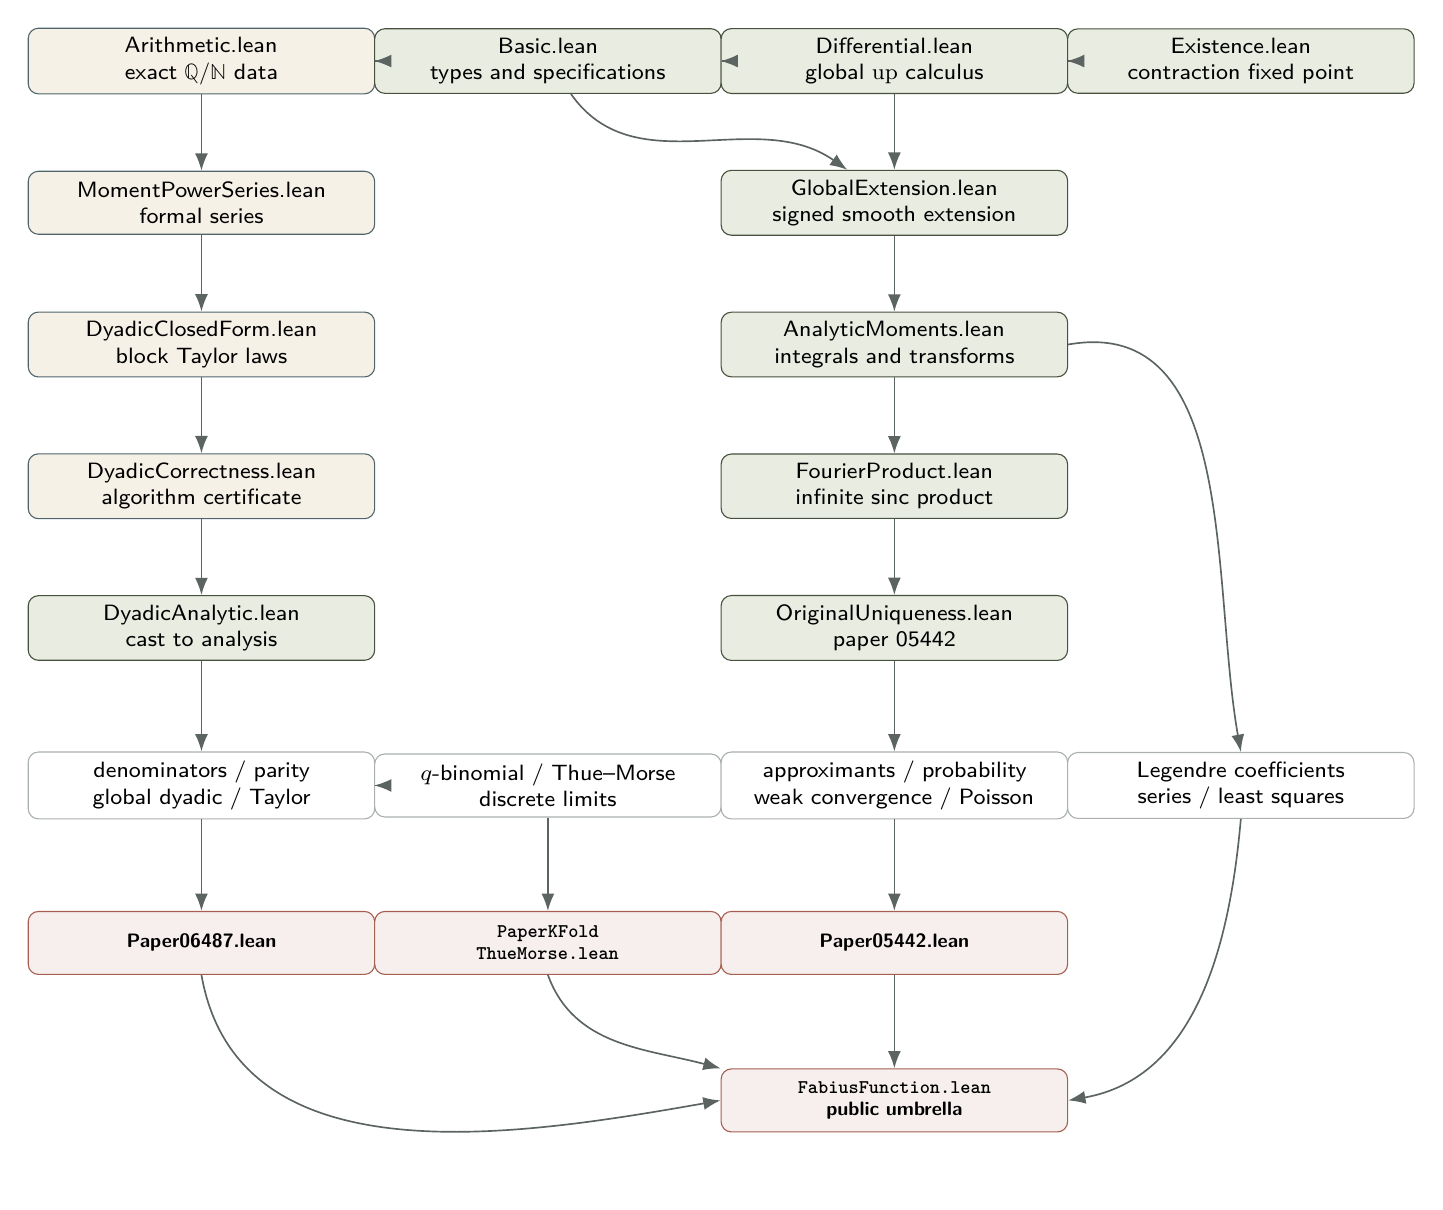
\begin{tikzpicture}[
  every node/.style={text width=3.8cm},
  mod/.append style={font=\sffamily\footnotesize},
  mathmod/.append style={font=\sffamily\footnotesize},
  generic/.append style={font=\sffamily\footnotesize},
  facade/.append style={font=\sffamily\scriptsize\bfseries}
]
  % Foundation row.
  \node[mathmod] (arith) at (0,0) {\module{Arithmetic}\\exact $\Q/\N$ data};
  \node[mod] (basic) at (4.4,0) {\module{Basic}\\types and specifications};
  \node[mod] (diff) at (8.8,0) {\module{Differential}\\global \upfun\ calculus};
  \node[mod] (exist) at (13.2,0) {\module{Existence}\\contraction fixed point};

  % Two mostly vertical proof spines: exact dyadic arithmetic and global analysis.
  \node[mathmod] (momps) at (0,-1.8) {\module{MomentPowerSeries}\\formal series};
  \node[mod] (global) at (8.8,-1.8) {\module{GlobalExtension}\\signed smooth extension};

  \node[mathmod] (dyclosed) at (0,-3.6) {\module{DyadicClosedForm}\\block Taylor laws};
  \node[mod] (moments) at (8.8,-3.6) {\module{AnalyticMoments}\\integrals and transforms};

  \node[mathmod] (dycorrect) at (0,-5.4) {\module{DyadicCorrectness}\\algorithm certificate};
  \node[mod] (fourier) at (8.8,-5.4) {\module{FourierProduct}\\infinite sinc product};

  \node[mod] (dyanalytic) at (0,-7.2) {\module{DyadicAnalytic}\\cast to analysis};
  \node[mod] (papers) at (8.8,-7.2) {\module{OriginalUniqueness}\\paper 05442};

  % Application families.
  \node[generic] (arith2) at (0,-9.2) {denominators / parity\\global dyadic / Taylor};
  \node[generic] (qbin) at (4.4,-9.2) {$q$-binomial / Thue--Morse\\discrete limits};
  \node[generic] (approx) at (8.8,-9.2) {approximants / probability\\weak convergence / Poisson};
  \node[generic] (leg) at (13.2,-9.2) {Legendre coefficients\\series / least squares};

  % Paper-facing aggregates and the public umbrella.
  \node[facade] (p2) at (0,-11.2) {\module{Paper06487}};
  \node[facade] (pk) at (4.4,-11.2) {\texttt{PaperKFold}\\\texttt{ThueMorse.lean}};
  \node[facade] (p1) at (8.8,-11.2) {\module{Paper05442}};
  \node[facade] (root) at (8.8,-13.2) {\texttt{FabiusFunction.lean}\\public umbrella};

  \draw[arrow] (arith)--(basic);
  \draw[arrow] (basic)--(diff);
  \draw[arrow] (diff)--(exist);

  \draw[arrow] (arith)--(momps);
  \draw[arrow] (momps)--(dyclosed);
  \draw[arrow] (dyclosed)--(dycorrect);
  \draw[arrow] (dycorrect)--(dyanalytic);

  \draw[arrow] (diff)--(global);
  \draw[arrow] (basic) to[out=-55,in=145] (global);
  \draw[arrow] (global)--(moments);
  \draw[arrow] (moments)--(fourier);
  \draw[arrow] (fourier)--(papers);

  \draw[arrow] (dyanalytic)--(arith2);
  \draw[arrow] (arith2)--(qbin);
  \draw[arrow] (papers)--(approx);
  \draw[arrow] (moments.east) to[out=10,in=100] (leg.north);

  \draw[arrow] (arith2)--(p2);
  \draw[arrow] (qbin)--(pk);
  \draw[arrow] (approx)--(p1);
  \draw[arrow] (p2.south) to[out=-80,in=190] (root.west);
  \draw[arrow] (pk.south) to[out=-70,in=165] (root.north west);
  \draw[arrow] (p1)--(root);
  \draw[arrow] (leg.south) to[out=-95,in=10] (root.east);
\end{tikzpicture}}
\caption{Selected dependency strata in the non-asymptotic development.}
\label{fig:core-dag}
\end{figure}

Three seams deserve special emphasis.

\begin{dependency}[title={Seam 1: arithmetic to analysis}]
\module{DyadicAnalytic} proves that the rational evaluator agrees with every
analytic object satisfying \decl{IsFabius}.  Once this is established, exact
arithmetic can be used in uniqueness, denominator, Legendre, and Taylor
arguments without reproving analytic formulas each time.
\end{dependency}

\begin{dependency}[title={Seam 2: local bump to global extension}]
\module{Differential} proves the smooth refinement equation for \upfun.
\module{GlobalExtension} combines that equation with local finiteness and
Thue--Morse reindexing.  Most global scaling identities depend on this seam,
not directly on the contraction construction.
\end{dependency}

\begin{dependency}[title={Seam 3: exact products to asymptotics}]
The asymptotic tower begins only after exact negative-Laplace product identities
are established.  Periodic regularization, Mellin constants, Lambert
coordinates, and saddle estimates are layered afterward.  This prevents
asymptotic approximations from contaminating exact algebraic rewrites.
\end{dependency}

\section{Why dependency direction matters}
A tempting informal development would define the canonical function first,
compute several values numerically, and then derive formulas from it.  This
library often reverses that order:
\begin{enumerate}
  \item define exact rational sequences independently;
  \item prove internal recurrence or power-series identities;
  \item certify an executable algorithm from an abstract recurrence;
  \item prove that analytic Fabius functions satisfy the same recurrence;
  \item conclude equality by induction or uniqueness.
\end{enumerate}
This direction is more modular.  The evaluator correctness theorem does not
know how the analytic function was constructed; the fixed-point construction
does not know the implementation details of the evaluator; and the canonical
specialization can be replaced without disturbing either side.

\section{Thin facades and thick bridges}
A rough rule for navigating the repository is:
\[
 \text{facade theorem}\longrightarrow
 \text{bridge theorem}\longrightarrow
 \text{generic infrastructure or exact core}.
\]
For example, a theorem displayed in \module{Paper06487} about a dyadic value
may be one line there, a substantial cast theorem in \module{GlobalDyadic}, a
closed rational identity in \module{DyadicClosedForm}, and a moment recurrence
in \module{MomentPowerSeries}.  The one-line facade is not “where the proof
is”; it is where the proof is \emph{named in the paper's vocabulary}.

\begin{readingpath}
For a first source tour, read
\module{Arithmetic} $\to$ \module{Basic} $\to$
\module{Differential} $\to$ \module{Existence} $\to$
\module{DyadicCorrectness} $\to$ \module{DyadicClosedForm} $\to$
\module{DyadicAnalytic} $\to$ \module{GlobalExtension}.
That sequence exposes almost every recurring design pattern before the larger
paper and asymptotic branches appear.
\end{readingpath}

% ================================================================================
\chapter{The exact arithmetic kernel}
\label{ch:arithmetic}

\section{Why \module{Arithmetic} comes first}
\module{Arithmetic} is mathematically elementary compared with the analytic
files, but architecturally it is foundational.  It defines objects over
$\N$, $\Z$, and $\Q$ that can be reduced by the kernel and evaluated without
choice, integration, limits, or real-number equality.  Its imports are kept
small enough that exact computation does not inherit the cost of the analytic
world.

The main families are:
\begin{description}
\item[Binary and Thue--Morse data.] \decl{binaryWeight} counts one-bits and
\decl{thueMorseSign} returns $(-1)^{s_2(n)}$.  Theorems for even and odd
indices are the reindexing engine used throughout the project.
\item[Moment sequences.] \decl{moment} and \decl{halfMoment} are rational
recurrences.  Their division-free companions \decl{momentNumerator} and
\decl{halfMomentNumerator} make integrality and parity induction possible.
\item[Closed dyadic formulas.] \decl{fabiusDyadic} is a finite exact sum for a
value at a dyadic argument; \decl{rvachevDyadic} and global signed versions
adapt it to other coordinates.
\item[Executable evaluation.] Tables of inverse-power values and a binary
Taylor/Horner descent evaluate a dyadic rational much faster than directly
expanding the closed sum.
\item[Denominator data.] Products of odd factors and Mersenne-type factors are
introduced in the exact type where divisibility statements belong.
\end{description}

\section{Binary identities are an API, not incidental lemmas}
The elementary rules
\[
 s_2(2n)=s_2(n),\qquad s_2(2n+1)=s_2(n)+1
\]
become sign rules
\[
 \TM(2n)=\TM(n),\qquad \TM(2n+1)=-\TM(n).
\]
In paper proofs these are often used silently.  Lean needs named theorems
because they drive reindexing under finite sums and infinite sums.  Later files
prove the stronger block-concatenation identity
\[
 \TM(h2^k+r)=\TM(h)\TM(r),\qquad 0\le r<2^k,
\]
which is the algebraic reason complete binary blocks cancel lower-degree
polynomials.

\begin{engineering}
The project consistently proves binary facts at the natural-number level and
casts their consequences afterward.  Trying to reason about bit counts after
casting indices to $\Q$, $\R$, or $\C$ would erase the structure Lean's
arithmetic and bitwise lemmas can see.
\end{engineering}

\section{Moments and division-free normalization}
The moment recurrence is naturally rational.  Divisibility and oddness,
however, are awkward when every induction step contains normalized fractions.
The code therefore maintains both the normalized sequence and a natural
numerator sequence.  Schematically,
\[
 c_n=\frac{A_n}{D_n},\qquad d_n=\frac{B_n}{E_n},
\]
where $A_n,B_n\in\N$ are defined recursively without division and $D_n,E_n$
are explicit factorial/Mersenne products.

This is a recurring formalization technique:
\begin{enumerate}
  \item state the mathematically natural recurrence in $\Q$;
  \item discover a common denominator from the recurrence;
  \item define a natural numerator by clearing that denominator;
  \item prove the rational sequence equals numerator divided by denominator;
  \item do parity, positivity, and divisibility on the natural sequence;
  \item transport the result back to $\Q$.
\end{enumerate}

The same split later supports \module{NormalizedMoments},
\module{NormalizedEvenMoments}, \module{HalfMomentDenominator},
\module{DenominatorBound}, and \module{TwoAdic}.

\section{The closed dyadic sum}
The definition \decl{fabiusDyadic} packages a finite Thue--Morse/moment formula.
Its exact displayed form is less important for navigating the source than its
role:
\begin{itemize}
  \item it is total on natural scale and numerator parameters;
  \item it is representation-stable under $(n,a)\mapsto(n+1,2a)$;
  \item its unit-interval cast is an analytic Fabius value;
  \item its global cast is a value of \decl{extendedFabius};
  \item its finite nature permits denominator and congruence arguments.
\end{itemize}

The library carefully distinguishes a \emph{closed specification} from an
\emph{algorithm}.  \decl{fabiusDyadic} is convenient for proofs because sums
can be rearranged and denominators exposed.  \decl{fabiusDyadicValue} is
convenient for execution because it follows the bits of the numerator.
\module{DyadicCorrectness} proves these two views coincide.

\section{The executable evaluator}
At scale $n$, the evaluator precomputes the values at inverse powers of two,
then descends through the nonzero bits of the numerator.  Conceptually, if the
highest active bit moves the argument into the neighboring dyadic block, the
function on that block is recovered from a finite Taylor polynomial whose
coefficients are earlier inverse-power values.  The implementation uses:
\begin{description}
\item[\decl{fabiusInversePowTwoTable}] a prefix table of exact rational values;
\item[\decl{fabiusTaylorHorner}] a Horner evaluator for the local Taylor
polynomial;
\item[\decl{fabiusDyadicUnitAux}] an auxiliary bit-clearing recursion;
\item[\decl{fabiusDyadicUnit}] the unit-interval algorithm;
\item[\decl{fabiusDyadicValue}] the public scale/numerator evaluator;
\item[\decl{evalFabiusDyadic}] a rational wrapper returning \code{Option ℚ},
rejecting non-dyadic rationals.
\end{description}

The README estimates the arithmetic shape as approximately
$O(n^2+n\,s_2(a))$: the table costs a triangular amount of exact work, and each
set bit triggers a Taylor/Horner block update.  Bit complexity also depends on
the rapidly growing rational numerators and denominators, so this estimate is
best read as a count of high-level rational operations.

\begin{proofidea}
The algorithm is not certified by unfolding it against the giant closed sum.
Instead the correctness layer asks for one abstract bit recurrence.  The closed
form proves that recurrence, and a strong-induction theorem then proves that
any table satisfying it agrees with the evaluator.  This is much closer to a
software-verification proof than to a direct symbolic calculation.
\end{proofidea}

% ================================================================================
\chapter{The specification and the differential bootstrap}
\label{ch:differential}

\section{\module{Basic}: the semantic vocabulary}
\module{Basic} imports the arithmetic kernel and enough analysis to state the
central objects.  It defines \decl{BoundedFabius}, \decl{fabiusReal},
\decl{IsFabius}, \decl{rvachevUp}, \decl{extendedFabius}, complex sinc, and
several transform-level definitions.  The file is intentionally definition
heavy: downstream modules should depend on a stable vocabulary rather than on
one existence proof.

A simplified view of the specification is:

\begin{LeanCode}
structure IsFabius (F : BoundedFabius) : Prop where
  zero_of_nonpos : ∀ x, x ≤ 0 → fabiusReal F x = 0
  one_of_one_le  : ∀ x, 1 ≤ x → fabiusReal F x = 1
  contDiff       : ContDiff ℝ ∞ (fabiusReal F)
  symmetry       : ∀ x ∈ Set.Icc (0 : ℝ) 1,
                     fabiusReal F x + fabiusReal F (1 - x) = 1
  hasDerivAt     : ∀ x ∈ Set.Icc (0 : ℝ) (1 / 2),
                     HasDerivAt (fabiusReal F)
                       (2 * fabiusReal F (2 * x)) x
\end{LeanCode}

The actual code chooses field formulations that interact smoothly with
mathlib's coercions and endpoint lemmas, but this excerpt captures the contract.
The rest of the library is mostly parametric in \code{F} and \code{hF}; the
canonical fixed point appears only when a theorem is specialized for end users.

\section{Folding to \upfun and managing the seam at zero}
The definition of \decl{rvachevUp} is piecewise at $x=0$.  Continuity is easy
from symmetry and endpoint values.  Differentiability is more delicate: Lean
must see that the left and right derivatives agree at the fold, and later that
all higher derivatives glue.

\module{Differential} proceeds in layers:
\begin{enumerate}
  \item prove evenness and support bounds directly from the branches;
  \item prove one-sided derivative formulas away from the fold;
  \item evaluate the boundary derivatives using flatness inherited from the
        constant tails and the Fabius differential equation;
  \item package a total \decl{HasDerivAt} theorem;
  \item bootstrap smoothness from the global derivative refinement equation.
\end{enumerate}

The resulting theorem has the recognizable form:

\begin{LeanCode}
theorem rvachev_hasDerivAt
    (F : BoundedFabius) (hF : IsFabius F) (x : ℝ) :
    HasDerivAt (rvachevUp F)
      (2 * (rvachevUp F (2 * x + 1) -
            rvachevUp F (2 * x - 1))) x := by
  ...
\end{LeanCode}

\section{Why the derivative formula bootstraps all smoothness}
The right side is a finite linear combination of affine compositions of
\decl{rvachevUp}.  Suppose $u$ is already $C^n$.  Then
$x\mapsto u(2x\pm1)$ is $C^n$, so the displayed formula says $u'$ is $C^n$.
The standard equivalence between $C^{n+1}$ regularity and a $C^n$ derivative
then gives $u\in C^{n+1}$.  Starting from continuity, induction yields
$C^\infty$.

The generic lemma
\decl{contDiff_of_hasDerivAt_dyadic_refinement} isolates this pattern.  It is
not limited to Rvachev's exact constants; it formalizes the reusable principle
“a continuously differentiable function whose derivative is a finite affine
combination of copies of itself is smooth.”

\begin{engineering}
This bootstrap avoids direct $n$th-derivative calculations at the piecewise
seam.  Proving every derivative glues by hand would duplicate endpoint
bookkeeping at each order.  Once the first global derivative identity is
established, the generic regularity lemma lets mathlib handle the induction.
\end{engineering}

\section{Support and positivity as analytic infrastructure}
The support theorem is not cosmetic.  Compact support turns \upfun into an
integrable function, a Schwartz function after complexification, and a safe
input to Poisson summation.  The library records both pointwise zero theorems
outside $[-1,1]$ and set-level support inclusions.  The set-level form is what
integration lemmas consume.

Strict positivity on $(-1,1)$ is proved later in
\module{Paper06487Supplement}.  Combined with the derivative identity it gives
strict increase on $(-1,0)$ and strict decrease on $(0,1)$.  This is a good
example of the project's layering: \module{Differential} proves the reusable
calculus statement; the paper supplement packages its elementary qualitative
consequences.

% ================================================================================
\chapter[Existence by contraction and uniqueness by dyadic density]{Existence by contraction and\\uniqueness by dyadic density}
\label{ch:existence}

\section{The fixed-point space}
\module{Existence} constructs the bounded Fabius function as a Banach fixed
point.  The ambient space is not all continuous functions $[0,1]\to\R$.
It is a closed subtype whose values lie in $[0,1]$ and whose members obey the
midpoint symmetry.  A schematic member $f$ satisfies
\[
 0\le f(x)\le1,
 \qquad f(x)+f(1-x)=1.
\]
The subtype is complete because it is closed in a complete sup-norm function
space.  Encoding symmetry in the space, rather than proving it after the fixed
point is found, makes the operator preserve an invariant that also produces
the contraction constant.

\section{The smoothing operator}
The construction extends a candidate to the real line with constant tails,
forms a cumulative integral, and folds/rescales it into another symmetric
unit-interval function.  The key numerical identity is that the total integral
of a symmetric candidate on $[0,1]$ is exactly $1/2$.  Indeed,
\[
 \int_0^1 f(t)\,dt
 =\frac12\int_0^1\bigl(f(t)+f(1-t)\bigr)\,dt
 =\frac12.
\]
That normalization ensures the transformed function has the correct endpoint
values without a candidate-dependent denominator.

The operator's Lipschitz estimate is exactly $1/2$.  On the first half of the
interval the difference of cumulative integrals is bounded by the interval
length times the sup norm.  On the second half, symmetry rewrites the estimate
back to the first.  Thus
\[
 \|Tf-Tg\|_\infty\le\frac12\|f-g\|_\infty.
\]
Mathlib's contraction fixed-point theorem yields a unique fixed candidate in
the subtype.

\begin{proofidea}
The factor $1/2$ is not an arbitrary weakened bound chosen to satisfy a
library theorem.  It is a structural consequence of doing all nontrivial
integration on a half interval and carrying symmetry as a type invariant.
This is why the choice of fixed-point space matters as much as the formula for
$T$.
\end{proofidea}

\section{Recovering the differential specification}
A fixed point of an integral operator first gives an integral equation.  The
file differentiates it on branch interiors and handles $0$, $1/2$, and $1$
with one-sided or gluing arguments.  The proof then invokes the differential
bootstrap of \module{Differential} to obtain $C^\infty$ regularity.  Finally the
constant tails are added to produce a value of \decl{BoundedFabius} and a proof
of \decl{IsFabius}.

The canonical declarations exposed through \module{PaperStatements} are
conceptually:

\begin{LeanCode}
noncomputable def fabius : BoundedFabius := ...

theorem fabius_spec : IsFabius fabius := ...

noncomputable def globalFabius : ℝ → ℝ :=
  extendedFabius fabius
\end{LeanCode}

\section{A second uniqueness layer}
Banach's theorem already gives uniqueness inside the fixed-point subtype.  The
public specification \decl{IsFabius}, however, is phrased by tails, symmetry,
smoothness, and a derivative equation.  The library proves that any function
satisfying that specification agrees with the fixed point.  The route is
not “show it is another fixed point and invoke Banach uniqueness.”  Instead it
uses the exact dyadic evaluator.

The proof has three stages.

\subsection{Stage 1: exact equality on every dyadic point}
\module{DyadicAnalytic} proves
\decl{fabiusDyadic_cast}: an abstract Fabius function at $a/2^n$ equals the
cast of \decl{fabiusDyadic}.  Hence two abstract solutions agree at every
dyadic point in $[0,1]$.

\subsection{Stage 2: approximate an arbitrary real by floor dyadics}
For $x\in[0,1]$, let
\[
 x_n=\frac{\lfloor 2^n x\rfloor}{2^n}.
\]
The standard bounds
\[
 0\le x-x_n<2^{-n}
\]
show $x_n\to x$.  Each $x_n$ lies in the allowed dyadic range and therefore
has the same value for both candidate functions.

\subsection{Stage 3: pass to the limit by continuity}
Both candidates are $C^\infty$, hence continuous.  Taking limits gives equality
at $x$.  Constant tails cover $x\notin[0,1]$.

\begin{engineering}
This proof makes the arithmetic evaluator part of the semantic uniqueness
story.  That may look circuitous, but it buys a valuable theorem: the exact
rational model is not merely a consequence of the canonical construction; it
characterizes every analytic solution on a dense set.
\end{engineering}

\section{What the final uniqueness API gives}
The file concludes with forms such as \decl{isFabius_eq},
\decl{existsUnique_fabius}, and an extensional equality theorem attached to the
specification.  Downstream code can therefore remain generic while knowing
that the parameter is propositionally unique.  In practice this is used in two
styles:
\begin{itemize}
  \item prove a theorem for arbitrary \code{F} and \code{hF}, then specialize
to \decl{fabius};
  \item construct an object by a different method, prove \decl{IsFabius}, and
identify it with the canonical object by uniqueness.
\end{itemize}
The probability CDF representation uses the second style.

% ================================================================================
\chapter{A second uniqueness theorem: the original compact-support problem}
\label{ch:original-uniqueness}

\section{The original specification includes an unknown scale}
The first Arias de Reyna paper starts from a compactly supported smooth
function $\varphi$ and a positive scale $k$ satisfying a two-scale derivative
identity.  The Lean predicate \decl{IsOriginalFabius} packages:
\begin{itemize}
  \item $C^\infty$ regularity;
  \item topological support exactly $[-1,1]$ or the corresponding support
        constraints used in the source;
  \item strict positivity in the interior;
  \item normalization $\varphi(0)=1$;
  \item a positive parameter $k$;
  \item the refinement equation for the derivative.
\end{itemize}
This problem is not identical to \decl{IsFabius}.  It asks Lean to recover both
the function and the scale.

For fidelity to the source, positivity remains a field of the predicate.  It is
logically redundant: \decl{IsOriginalFabius.mk_of_derivative_law} derives it
from the other five hypotheses by applying the mean-value theorem on
$[-1,0]$, where support removes one translated term and interior positivity
fixes the sign of the other.

\section{First force the scale to be two}
\module{OriginalCharacterization} derives endpoint values, a two-term partition
identity, and total integral one.  Integrating or evaluating the refinement
law against these normalizations forces $k=2$.  The exact route is arranged so
that support removes translated terms and the remaining integral identities
can be discharged without assuming the desired value in advance.

Once $k=2$, the canonical \decl{rvachevUp fabius} is shown to satisfy the
original predicate.

\section{Fourier uniqueness in Schwartz space}
\module{OriginalUniqueness} proves uniqueness by a route independent of the
fixed-point/dyadic-density argument.

Because $\varphi$ is smooth and compactly supported, its complexification is a
Schwartz map.  Fourier transforming the differential refinement equation gives
a multiplicative recurrence.  After normalization at frequency zero, one
obtains a sinc factor:
\[
 \widehat\varphi(\xi)
   =\operatorname{sinc}(\pi\xi)\,
      \widehat\varphi(\xi/2),
\]
after matching the project's Fourier convention.  Iteration gives
\[
 \widehat\varphi(\xi)=
   \left(\prod_{j=0}^{N-1}
      \operatorname{sinc}\!\left(\frac{\pi\xi}{2^j}\right)\right)
   \widehat\varphi(\xi/2^N).
\]
As $N\to\infty$, continuity and normalization imply the last factor tends to
one.  Therefore every original solution has the same infinite sinc product as
the canonical \upfun.  Injectivity of the Fourier transform on Schwartz space
then gives equality of the functions.

\begin{proofidea}
The proof uses compact support twice: first to package the function as Schwartz,
and second to ensure the Fourier transform has all the regularity and decay
needed by the injectivity theorem.  The infinite product is not guessed; it is
the limit of a finite recurrence whose remainder frequency tends to zero.
\end{proofidea}

\section{Why both uniqueness proofs belong in the library}
The two routes solve different interface problems.
\begin{description}
\item[Dyadic-density uniqueness] identifies all bounded cumulative solutions of
\decl{IsFabius}.  It emphasizes exact arithmetic and continuity.
\item[Fourier uniqueness] identifies all compactly supported smooth original
solutions and determines the unknown scale.  It emphasizes transform theory
and support.
\end{description}
Neither is redundant.  The first certifies exact computation as a complete
dense fingerprint; the second mirrors the original mathematical
characterization and builds infrastructure later reused for the Fourier product
and Poisson summation.

% ================================================================================
\chapter[Formal power series and analytic moments]{Formal power series and\\analytic moments}
\label{ch:moments}

\section{The formal-series layer is deliberately pre-analytic}
\module{MomentPowerSeries} proves the moment recurrences as identities in
formal power series.  This removes all radius-of-convergence and interchange
questions.  A representative identity rescales the moment series and factors
it through a hyperbolic-sine quotient:
\[
 M(4X)=M(X)\,\frac{\sinh\sqrt{X}}{\sqrt{X}},
\]
with the precise indexing and normalization encoded by the project's
\decl{momentPS} and auxiliary series.  The point is structural: coefficient
extraction from a formal product exactly reproduces the finite recurrence.

The half-moment series is then characterized by another functional equation.
The file constructs a candidate, proves the functional equation, and proves
uniqueness coefficient by coefficient with strong induction.  Even/odd
coefficient filtering yields the key relations among \decl{moment},
\decl{halfMoment}, and inverse-power Fabius values.

\begin{engineering}
When an identity is fundamentally coefficient algebra, the code stays in
\code{PowerSeries ℚ}.  Analytic convergence appears only in modules whose
conclusions are genuinely about functions, integrals, or transforms.  This
separation makes recurrence proofs faster, more exact, and much easier to
reuse in denominator arguments.
\end{engineering}

\section{From the bump to integral moments}
\module{AnalyticMoments} begins on the analytic side.  Compact support and
evenness permit all whole-line integrals to be localized.  The normalization
\[
 \int_{\R}\upfun_F(x)\,dx=1
\]
is derived from the differential/refinement equation rather than installed as
an axiom.

Integration by parts then converts the derivative equation into moment
recurrences.  The boundary terms vanish because of compact support and
flatness.  For even powers, symmetry kills odd contributions and leaves the
same rational recurrence used by \decl{moment}.  Uniqueness of the recurrence
identifies the integral with the exact sequence:
\[
 \int_{-1}^{1} x^{2n}\upfun_F(x)\,dx=c_n.
\]
A half-interval version similarly identifies \decl{halfMoment}.  The additive
theorem \pathbreak{halfMoment_eq_integral_formula_all} includes the normalized
zeroth term, where both exact and analytic definitions equal one, without
changing the source-faithful positive-index theorem.

\section{The inverse-power identity}
One of the most important bridges in the library relates the value at
$2^{-n}$ to a half moment.  In normalized schematic form,
\[
 F(2^{-n})=
 \frac{d_n}{n!\,2^{\binom n2}},
\]
where $d_n$ is the project's \decl{halfMoment n} up to the exact indexing used
in the declaration.  This theorem appears in multiple useful forms:
\begin{itemize}
  \item an exact rational identity in \module{MomentPowerSeries};
  \item a real analytic formula for arbitrary \code{F} and \code{hF};
  \item a table-entry theorem used by the executable evaluator;
  \item a denominator/valuation input;
  \item a coefficient source for Legendre expansions.
\end{itemize}

The declaration \pathbreak{halfMomentFabiusValue} packages the rational normalization,
while \pathbreak{fabiusAtInverseTwoPow_eq_halfMoment} and cast variants connect it to
the function.

\section{Generating functions, Laplace transforms, and Fourier transforms}
Once moments are integrals, exponential series can be interchanged with the
compactly supported integral.  The code obtains generating-function and
Laplace identities by dominated convergence or standard integral-series
lemmas.  Complexification yields the Fourier transform at complex arguments,
which is later identified with the infinite sinc product.

A useful navigation rule is:
\begin{itemize}
  \item \module{MomentPowerSeries}: exact coefficient algebra;
  \item \module{AnalyticMoments}: integral identification and transform series;
  \item \module{LaplaceTransform}, \module{LaplaceMoments}: transform-specific
        packaged theorems;
  \item \module{FourierAnalytic}, \module{FourierProduct}: entire/Fourier
        consequences and product evaluation.
\end{itemize}

\section{Normalized moments and denominator chains}
\module{NormalizedMoments} and \module{NormalizedEvenMoments} make common
denominators explicit.  A typical proof proceeds by induction on the recurrence,
using the fact that earlier denominator products divide later ones.  The
normalizing product is chosen to be multiplicative and monotone under index,
which lets Lean combine divisibility witnesses mechanically.

\module{HalfMomentDenominator} sharpens the half-moment normalization.
\module{TwoAdic} then proves parity of the normalized numerator, often by
showing that all but one term in a recurrence are even and identifying the
surviving Pascal-row contribution.  The resulting $2$-adic valuations are
statements about exact rationals, not numerical experiments.

% ================================================================================
\chapter[Certified exact evaluation at dyadic rationals]{Certified exact evaluation\\at dyadic rationals}
\label{ch:dyadic}

\section{Four files, four proof obligations}
The evaluator story is split across four central modules.

\begin{longtable}{@{}>{\raggedright\arraybackslash}p{.33\textwidth}p{.60\textwidth}@{}}
\toprule
Module & Responsibility \\
\midrule
\endhead
\module{Arithmetic} & Define the closed sum, inverse-power table, Horner
routine, bit recursion, and public exact evaluator. \\
\module{DyadicCorrectness} & Prove representation stability and show that an
abstract bit recurrence is sufficient for implementation correctness. \\
\module{DyadicClosedForm} & Derive the needed bit/block recurrence from
Thue--Morse cancellation and polynomial/Taylor algebra. \\
\module{DyadicAnalytic} & Prove that every analytic Fabius function obeys the
same recurrence and identify its values with the rational evaluator. \\
\bottomrule
\end{longtable}

This decomposition prevents a cyclic proof.  The algorithm is specified before
analysis; the closed rational formula is proved correct without using the
canonical function; the analytic function is linked only after both exact
pieces are stable.

\section{Representation refinement}
A dyadic number has infinitely many scale/numerator representations:
\[
 \frac{a}{2^n}=\frac{2a}{2^{n+1}}=\frac{4a}{2^{n+2}}=\cdots.
\]
Before a public rational evaluator can be trusted, the code proves that its
value is invariant under this refinement.  This theorem is separate from
function correctness.  It says that the implementation computes a
well-defined function of the dyadic rational, rather than a function of a
chosen encoding.

The wrapper \decl{evalFabiusDyadic} analyzes a rational denominator and returns
\code{none} precisely when it is not a power of two after reduction.  Its
correctness API includes both directions: accepted inputs have a certified
exact value, and rejected inputs are genuinely non-dyadic.

\section{Prefix stability of the inverse-power table}
The inverse-power table is built incrementally.  Later scales append entries
but must not alter earlier ones.  \module{DyadicCorrectness} proves:
\begin{itemize}
  \item the exact table length;
  \item an append recurrence for the next inverse-power value;
  \item lookup stability under extension;
  \item Horner evaluation invariants for prefixes;
  \item compatibility between auxiliary and public evaluators.
\end{itemize}
These are ordinary program invariants, and their separation from the
mathematical recurrence is exemplary.  A change in table representation would
mostly affect this file, not the analytic bridge.

\section{The abstract bit recurrence}
The central interface is a predicate of the form
\decl{FabiusDyadicHasBitRecurrence}.  Informally it says: when the highest
nonzero bit of the numerator is removed, the value in the corresponding
binary block is obtained by a finite Taylor expression using the inverse-power
table.  The exact predicate carries the necessary range and scale conditions.

A strong-induction theorem then has the shape:

\begin{LeanCode}
theorem fabiusDyadicUnit_eq_of_hasBitRecurrence
    (table : List ℚ)
    (hrec : FabiusDyadicHasBitRecurrence table) :
    ∀ n a, ... →
      fabiusDyadicUnit table n a = fabiusDyadic n a := by
  intro n a
  induction a using Nat.strong_induction_on with
  | h a ih =>
      -- clear the highest bit; recursive arguments are smaller
      ...
\end{LeanCode}

The proof follows the executable control flow.  The recursion is justified not
by decreasing scale but by decreasing numerator after clearing a set bit.
That is why strong induction on $a$, rather than ordinary induction on $n$, is
the natural principle.

\section{Thue--Morse cancellation creates Taylor blocks}
\module{DyadicClosedForm} supplies the mathematical recurrence.  Its first
major ingredient is the Prouhet cancellation identity
\[
 \sum_{r=0}^{2^b-1}(-1)^{s_2(r)}r^d=0
 \qquad(d<b),
\]
and the normalized nonzero value at $d=b$.  The file proves affine and
translated variants, because the dyadic closed form contains powers of shifted
indices rather than bare $r^d$.

The second ingredient is a polynomial kernel whose Hasse derivatives encode
local Taylor coefficients.  A refinement identity is established by showing
that the derivatives of two polynomials agree and their constant terms agree.
This is often more robust in Lean than expanding both sides into enormous
binomial sums.

Complete binary blocks annihilate all powers below the critical degree.  What
survives is exactly the coefficient needed for the next inverse-power table
entry.  Partial blocks produce a Taylor polynomial.  These facts are packaged
as a block Taylor property, then converted to the abstract bit recurrence.

\begin{proofidea}
The highest-bit step works because binary concatenation factors the Thue--Morse
sign and because a complete $2^b$ block acts like a finite-difference operator
of order $b$.  Lower-degree Taylor terms cancel; the first nonzero term has a
closed normalization.  The evaluator is therefore a compressed traversal of
the same cancellation already present in the closed formula.
\end{proofidea}

\section{The analytic recurrence}
\module{DyadicAnalytic} independently proves a Taylor-block recurrence for any
\code{F} satisfying \decl{IsFabius}.  The key analytic input is the iterated
derivative scaling law, eventually available in global form:
\[
 \widetilde F^{(k)}(x)
 =2^{\binom{k+1}{2}}\widetilde F(2^k x).
\]
At dyadic base points these derivatives are inverse-power values already in the
table.  A finite Taylor formula is exact on the relevant block because the
translated remainder cancels by the signed scale-translation identity; in the
local unit-interval proof, the same effect is obtained through the refinement
recurrence.

The file proves the first scale separately, then inducts through higher scales.
It identifies the analytic Taylor sum with the cast of
\decl{fabiusTaylorHorner}, proves the bit recurrence, and applies the same
strong-induction framework used by the exact closed form.  The final theorem is
\decl{fabiusDyadic_cast}.

\section{Why this is a particularly strong formalization result}
The result is more than “the first few dyadic values are rational.”  It gives:
\begin{itemize}
  \item a total exact algorithm for every dyadic rational in the domain;
  \item proof that different encodings give the same answer;
  \item proof that the algorithm equals a closed finite formula;
  \item proof that the exact result equals every analytic solution;
  \item exact denominator and valuation consequences downstream.
\end{itemize}
The code thus joins executable mathematics, algebraic combinatorics, and
functional analysis at a single certified interface.

% ================================================================================
\chapter{The signed global extension and dyadic translation calculus}
\label{ch:global}

\section{Local finiteness hidden inside a \texttt{tsum}}
The definition
\[
 \widetilde F(x)=\sum_{n\ge0}\TM(n)\upfun_F(x-2n-1)
\]
uses a topological sum because that is the natural public expression.  Yet the
support of \upfun means the summand can be nonzero only when
\[
 -1<x-2n-1<1,
\]
so at each fixed $x$ at most one or two neighboring indices matter, depending
on endpoint convention.  On a sufficiently small neighborhood the same finite
set of indices works uniformly.

\module{GlobalExtension} converts this observation into local finite-sum
equalities.  The proof pattern is:
\begin{enumerate}
  \item choose integer bounds from the point $x$ and a small radius;
  \item prove all indices outside a finite range evaluate outside the support;
  \item rewrite the \code{tsum} as a finite \code{Finset.sum};
  \item apply finite-sum continuity or smoothness;
  \item transfer the local result back to \decl{extendedFabius}.
\end{enumerate}
This is more robust than trying to prove uniform summability of all derivatives
for a series that is actually locally finite.

\section{Agreement with the bounded coordinate}
For $x\in[0,1]$, only the first translated bump contributes, and its branch is
exactly the bounded cumulative function.  The file proves
\decl{extendedFabius_eq_fabiusReal} on the closed unit interval.  For $x\le0$,
all translates lie outside support and \decl{extendedFabius_eq_zero_of_nonpos}
provides flatness at the origin.

A block-local theorem identifies the unique surviving translate on intervals
of length two.  This is the basic simplifier used in global dyadic and
translation proofs: instead of unfolding a global infinite sum, choose the
block containing $x$ and reduce to one \upfun value with a Thue--Morse sign.

\section{Reindexing the derivative}
Differentiate termwise after replacing the series locally by a finite sum.
Each bump derivative contributes
\[
 2\upfun_F(2x-4n-1)-2\upfun_F(2x-4n-3).
\]
The two families correspond to even and odd indices in the extension evaluated
at $2x$.  The identities
\[
 \TM(2n)=\TM(n),\qquad \TM(2n+1)=-\TM(n)
\]
make the signs align, yielding
\[
 \widetilde F'(x)=2\widetilde F(2x).
\]
In Lean, the hard part is not differentiation but exact reindexing of two
locally finite sums.  The file supplies explicit even/odd bijections and uses
support to justify the chosen finite ranges.

\section{The closed formula for all iterated derivatives}
Repeated differentiation gives the triangular power of two
\[
 \widetilde F^{(k)}(x)
 =2^{1+2+\cdots+k}\widetilde F(2^k x)
 =2^{\binom{k+1}{2}}\widetilde F(2^k x).
\]
The formal theorem is named \decl{iteratedDeriv_extendedFabius}.  The induction
must reconcile three pieces of syntax:
\begin{itemize}
  \item \code{iteratedDeriv (k+1)} as a derivative of
        \code{iteratedDeriv k};
  \item the chain-rule factor $2^k$ from differentiating $x\mapsto2^kx$;
  \item the combinatorial identity
        $\binom{k+2}{2}=\binom{k+1}{2}+k+1$.
\end{itemize}
This theorem is one of the most reused declarations in the subtree.  It feeds
Taylor reduction, inverse-power identities, flatness, translated splines, and
endpoint asymptotics.

\section{Power-of-two translation and Thue--Morse sign change}
\module{ScaleTranslation} proves that on the initial block,
\[
 \widetilde F(x+2^r)=-\widetilde F(x),
 \qquad 0\le x\le2^r,
\]
for $r\ge1$.  The proof truncates both global sums to finite ranges.  The
translated range is the next binary block, and the binary weight identity
\[
 s_2(2^{r-1}+m)=s_2(m)+1
 \qquad(0\le m<2^{r-1})
\]
flips every sign.  The support arguments ensure that no other translates
survive.

Combining translation with the iterated derivative formula gives a sign change
for sufficiently high derivatives translated by a dyadic scale, even when the
scale is an integer rather than a natural.  This is the technical form needed
by Taylor remainder cancellation.

\section{Exact cancellation of neighboring Taylor remainders}
Suppose $x$ lies in the dyadic annulus
\[
 2^s\le x<2^{s+1}.
\]
Write $x=2^s+y$ with $0\le y<2^s$.  The integral remainder in the Taylor
expansion about $2^s$ is transformed by $t\mapsto t+2^s$.  The derivative
translation theorem changes its sign, and the polynomial kernel
$(x-t)^n$ becomes $(y-t)^n$.  Therefore the remainder about $2^s$ is the
negative of the remainder about zero at $y$.

\module{TaylorReduction} combines the two Taylor formulas.  Since every
iterated derivative of \decl{extendedFabius} vanishes at zero, the expansion at
zero consists only of the remainder.  The expansion at the inverse-power base
has coefficients expressible through half moments.  Adding the equations
cancels the remainders and yields a \emph{finite exact} reduction formula.

\begin{LeanCode}
theorem extendedFabius_reduction
    (F : BoundedFabius) (hF : IsFabius F)
    (x : ℝ) (n : ℤ)
    (hx : 0 < x)
    (hlo : (2 : ℝ) ^ (-n) ≤ x)
    (hhi : x < (2 : ℝ) ^ (-n + 1)) :
    let y := x - (2 : ℝ) ^ (-n)
    extendedFabius F x = -extendedFabius F y +
      if 0 ≤ n then fabiusReductionSum n.toNat y else 0 := by
  ...
\end{LeanCode}

For nonnegative $n$, the finite sum is a moment-normalized Taylor polynomial.
For negative $n$, the statement reduces directly to the power-of-two sign
translation law and the correction term is zero.

\begin{proofidea}
The formula is exact despite using Taylor's theorem because the remainder is
not estimated; it is paired with an adjacent remainder and canceled by a
Thue--Morse translation identity.  This “Taylor expansion plus exact remainder
symmetry” is a signature technique of the arithmetic paper branch.
\end{proofidea}

% ================================================================================
\chapter{The first paper facade: compact support, probability, and approximation}
\label{ch:paper05442}

\section{What \module{Paper05442} exposes}
\module{Paper05442} is the facade for Juan Arias de Reyna's
\emph{An infinitely differentiable function with compact support: definition
and properties}.  It imports:
\begin{itemize}
  \item \module{OriginalUniqueness} for Theorem 1;
  \item \module{WeakConvergence} for the early probability measures;
  \item \module{StepApproximationLimit} for the pointwise finite-step limit;
  \item \module{ProbabilityRepresentation} for the infinite product model;
  \item \module{PoissonSummation} for partitions of unity;
  \item \module{OriginalPaperSupplement} for prose-level identities and
        corrected forms not represented as numbered theorem environments.
\end{itemize}
The facade is best read beside the paper.  The lower modules are best read when
trying to understand or extend a proof.

\section{Finite convolution and atomic approximants}
\module{EarlyApproximants} builds finite probability measures from centered
Bernoulli or uniform ingredients at dyadically shrinking scales.  Their
characteristic functions are finite products of cosine or sinc factors, the
finite analogues of the Fourier product of \upfun.

The same coefficients are repackaged as step functions.  Half-weighted endpoint
indicators are used so that convolution identities remain correct at jump
points.  This detail matters: ordinary closed or open interval indicators give
the right function almost everywhere but fail at the exact endpoints where the
paper states pointwise identities.

\begin{correction}
The formalization records two source-level repairs.  The equation corresponding
to the finite convolution must use the finite convolution object actually
defined at that stage, and the step approximation theorem needs half weights at
cell endpoints.  These are not measure-theoretic quibbles: without them the
literal pointwise formula is false on a finite set.
\end{correction}

\section{From interval averages to pointwise convergence}
\module{StepApproximationLimit} proves convergence without differentiating the
step functions.  First it establishes coefficient unimodality, which gives
monotonicity on one side of the center and antitonicity on the other.  Then it
proves convergence of integrals over intervals.  A generic squeezing theorem
says, roughly:

\begin{quote}
If monotone approximants have convergent integrals over every sufficiently
small interval and the limiting density is continuous, then the pointwise
values converge to the density.
\end{quote}

For a monotone function, the value at a point is trapped between the left and
right interval averages.  As the interval shrinks, continuity makes both
limiting averages approach the same value.  The file packages this argument so
that the final theorem
\decl{stepApproximant_tendsto_rvachevUp} is a clean specialization.

\begin{engineering}
The generic interval-average lemma is stronger and cleaner than a proof tied to
the explicit coefficients.  All coefficient combinatorics is discharged
before the limiting argument begins.  This is a common pattern in the project:
make the final analytic convergence theorem depend on a compact abstract
interface.
\end{engineering}

\section{Weak convergence through characteristic functions}
\module{WeakConvergence} treats the corresponding probability measures.  The
finite characteristic function is a product over the first $n$ dyadic scales.
The target characteristic function is the infinite sinc product associated
with \upfun.

The proof separates a finite head and an infinite tail.  The head converges by
literal stabilization.  For the tail, a local estimate
\[
 \operatorname{sinc}(z)=1+O(z^2)
\]
and the geometric sum of squared dyadic scales show the omitted product tends
to one.  In the finite approximants an additional exponent $n$ appears; the
relevant elementary limit is of the form $n2^{-n}\to0$.

Once pointwise convergence of characteristic functions and continuity at zero
are established, mathlib's Lévy continuity theorem gives weak convergence of
probability measures.  The file also exports the bounded-continuous test
function formulation, which is often more useful downstream than the abstract
measure topology statement.

\section{The infinite product probability representation}
\module{ProbabilityRepresentation} gives a different construction.  Its sample
space is
\[
 \Omega=[0,1]^{\N}
\]
with product Lebesgue probability measure, represented in Lean as functions
\code{ℕ → Set.Icc (0 : ℝ) 1}.  Define
\[
 X(\omega)=\sum_{n=0}^{\infty}\frac{\omega_n}{2^{n+1}}.
\]
Uniform convergence against the geometric majorant gives continuity and
measurability.  Pointwise bounds show $0\le X\le1$.

The head/tail decomposition is exact:
\[
 X(\omega)=\frac{\omega_0+X(\operatorname{tail}\omega)}2.
\]
The code proves that the first coordinate and the tail process are independent,
that deleting the first coordinate preserves the product measure, and hence
that the law $\mu$ of $X$ is self-similar:
\[
 \mu=(\lambda_{[0,1]}\times\mu)\circ
       \left((u,v)\mapsto\frac{u+v}{2}\right)^{-1}.
\]

\section{The CDF satisfies the Fabius smoothing equation}
Let $H(y)=\mu(( -\infty,y])$.  Conditioning on the first uniform coordinate
gives
\[
 H(y)=\int_0^1 H(2y-u)\,du.
\]
The Lean proof is explicit: rewrite the CDF as a measure of a measurable set,
use the map equation for $\mu$, apply product integration/Fubini to the
indicator, and identify each fiber measure with $H(2y-u)$.

Coordinatewise reflection $\omega_n\mapsto1-\omega_n$ preserves product
measure and sends $X$ to $1-X$.  Therefore $H(y)+H(1-y)=1$ on $[0,1]$.
Differentiating the smoothing equation or using the cumulative operator shows
that $H$ satisfies \decl{IsFabius}.  The uniqueness theorem from
\module{Existence} then identifies $H$ with \decl{fabiusReal fabius}.

\begin{proofidea}
Probability is used as an alternative construction, not as an assumption about
the canonical fixed point.  The law is built first; self-similarity yields the
same analytic specification; uniqueness supplies identification.  This keeps
the probabilistic representation honest and modular.
\end{proofidea}

\section{Fourier product and Poisson summation}
\module{FourierProduct} defines complex sinc as the divided slope of sine at
zero, making it an entire function without a special-case singularity in later
analytic theorems.  Local estimates prove convergence of
\[
 \prod_{n\ge0}\operatorname{sinc}
     \!\left(\frac{\pi z}{2^n}\right)
\]
uniformly on compact subsets.  The Fourier refinement recurrence produces the
finite product; the residual transform at $z/2^N$ tends to its value at zero,
which is one.  Thus the Fourier transform of \upfun is exactly the infinite
product.

For Poisson summation, \module{PoissonSummation} packages a positively rescaled
\upfun as a Schwartz map and computes its Fourier transform under scaling.
The same construction exposes
\pathbreak{rvachevFourier_real_iteratedDeriv_rapidDecay}: for every pair of
natural indices, an arbitrary polynomial frequency weight times the
corresponding real-axis derivative is uniformly bounded.  Its specialization
\pathbreak{rvachevFourier_real_rapidDecay} is the rapid decay of the transform
itself.
Mathlib's Schwartz Poisson theorem then gives
\[
 \sum_{k\in\Z}\upfun_F(t+uk)
 =\frac1u\sum_{k\in\Z}
   \widehat{\upfun_F}(k/u)
   e^{2\pi i k t/u}
 \qquad(u>0).
\]
The sinc product vanishes at every nonzero integer because its first factor
already vanishes.  Taking $u=1/n$ leaves only the zero Fourier mode and yields
\[
 \sum_{k\in\Z}\upfun_F\left(t+\frac{k}{n}\right)=n.
\]
In particular, integer translates form a partition of unity.

\begin{correction}
The printed exponential in equation (25) of the source omits its dependence on
$t$.  The formal theorem includes
$e^{2\pi i k t/u}$, as forced both by Poisson summation and by the later
specialization.  The module also records a correction to equation (32): after
multiplying the preceding identity by the scale parameter, the displayed
factor $1/a$ must disappear.
\end{correction}

% ================================================================================
\chapter{The arithmetic paper facade}
\label{ch:paper06487}

\section{Numbered statements versus prose-level support}
\module{Paper06487} exposes the numbered results of
\emph{Arithmetic of the Fabius function}.  Most theorem bodies are short
applications of \module{PaperStatements} and
\module{Paper06487Supplement}.  The latter collects claims used in prose or in
proofs but not set off as numbered theorem environments.

This split is useful for maintenance:
\begin{itemize}
  \item \module{PaperStatements} is the stable numbered API;
  \item \module{Paper06487Supplement} records exact auxiliary assertions,
        corrections, and expanded displayed formulas;
  \item lower modules remain organized by mathematical mechanism rather than
        paper order.
\end{itemize}

\section{Qualitative consequences}
The supplement proves nonnegativity of all moments from their exact recurrence,
strict positivity of \upfun on the interior of its support, and signs of its
derivative on the two halves.  It also exposes the elementary identity
\[
 \upfun_F(t)+\upfun_F(1-t)=1\qquad(0\le t\le1),
\]
which follows by reducing each branch to bounded Fabius symmetry.

Every derivative of \decl{extendedFabius} vanishes at zero.  More generally,
for positive integer scale, all derivatives vanish at $2^s$.  The proof uses
the iterated derivative formula and the power-of-two sign translation at the
origin.  These flatness results justify exact Taylor manipulations that would
otherwise leave endpoint terms.

\section{Global dyadic formulas}
\module{GlobalDyadic} transports the unit-interval exact formula to the signed
extension.  A real dyadic point is reduced to a length-two block, the unique
surviving translate is identified, and the Thue--Morse sign of the block is
factored out.  This is the global analogue of representation refinement:
different block/scale decompositions must give the same rational value.

The supplement presents the “shifted Rvachev” formula in both compact and fully
expanded forms.  For an integer $a$ in the allowed range,
\[
 \upfun_F\!\left(\frac{a-2^n}{2^n}\right)
   =\operatorname{fabiusDyadic}(n,a),
\]
then unfolds the right side into the paper's finite double sum.  Keeping both
forms is valuable: the compact theorem rewrites well; the expanded theorem
matches a printed formula exactly.

\section{Denominator bounds}
\module{DenominatorBound} starts from the exact finite dyadic formula.  It
chooses an explicit common denominator, multiplies the sum by it, and proves
the result is a natural number.  From
\[
 D\cdot q\in\Z
\]
for a reduced rational $q$, a generic rational lemma concludes that the
reduced denominator of $q$ divides $D$.  Taking a least common multiple over a
finite dyadic grid gives the paper's denominator bound.

The proof is organized to avoid direct manipulation of
\code{Rat.den}: all complicated algebra is done before reduction, while a small
generic theorem handles the final divisibility consequence of reduced form.

\section{Odd normalizations and \texorpdfstring{$2$-adic}{2-adic} valuations}
\module{TwoAdic} proves that certain normalized moment numerators are odd.  The
main recurrence argument separates terms by parity and uses exact facts about
binomial coefficients.  Once a rational is written as an odd integer divided
by an explicit power of two times odd factors, \code{padicValRat 2} simplifies
to the visible exponent.

The paper supplement records a corrected proof-internal factor: in a theorem-20
normalization, the natural quantity is $2d_kN_n$, not $d_kN_n$.  The Lean theorem
states the corrected product and then strengthens it to an odd natural number.
This correction propagates cleanly because normalization facts are isolated
from the final numbered theorem.

\begin{correction}
The arithmetic facade does not silently “make the proof go through.”  Where a
printed sentence omits a factor or a lemma needs an extra range hypothesis, the
source comment names the discrepancy and the public declaration states the
repair.  This turns the formalization into an auditable critical edition of the
mathematics.
\end{correction}

\section{Taylor reduction as the computational heart of the paper}
Proposition 10's recursive formula is assembled from
\module{ScaleTranslation}, \module{TaylorReduction}, inverse-power values, and
flatness.  It reduces an argument in one dyadic annulus to a smaller translated
argument plus an explicit polynomial in the displacement.  Iterating the
reduction follows the binary expansion of the argument, which explains the
close relationship between the paper formula and the exact bit evaluator.

The formalization has two advantages over a purely handwritten recursion:
\begin{itemize}
  \item integer scales make the negative-index branch explicit rather than
        tacitly assuming the argument is below one;
  \item every use of Taylor's theorem carries its domain, differentiability,
        and interval-integrability hypotheses, so endpoint flatness cannot be
        accidentally omitted.
\end{itemize}

% ================================================================================
\chapter{Thue--Morse generating identities and \texorpdfstring{$q$-binomial}{q-binomial} formulas}
\label{ch:qbinomial}

\section{The combinatorial sublibrary}
The exact formulas beyond the two papers depend on a substantial Thue--Morse
sublibrary:
\begin{description}
\item[\module{ThueMorsePrefix}] finite prefixes, parity splitting, block sums,
and iterated prefix convolution;
\item[\module{ThueMorseGenerating}] polynomial and formal generating
identities;
\item[\module{ThueMorseExponential}] finite exponential sums and their binary
product factorization;
\item[\module{ThueMorseApproximation}] corrected approximation statements and
error bounds;
\item[\module{ThueMorseBinomialLog}] the zero--one sequence, binomial parity,
and exact base-two logarithm formulas;
\item[\module{HalfQBinomial}] Gaussian binomial coefficients at $q=1/2$ and
finite Pochhammer products.
\end{description}
These modules are not merely support code for one formula.  They make the
binary cancellation mechanisms reusable in discrete limits, splines, and
asymptotic comparison results.

\section{Finite exponential factorization}
For a binary prefix of length $2^n$, the signed exponential sum factors:
\[
 \sum_{r=0}^{2^n-1}\TM(r)e^{rz}
   =\prod_{j=0}^{n-1}\bigl(1-e^{2^jz}\bigr).
\]
The proof is an induction that splits the next block into even and odd halves.
The sign rules turn the odd half into a negative shifted copy of the even half,
producing the next factor.  Differentiating or extracting coefficients gives
the Prouhet power-sum cancellation used in the dyadic and spline branches.

\section{\texorpdfstring{$q$-weights}{q-weights} as coefficient extractors}
\module{FabiusQBinomialFormula} is a large algebraic bridge.  Its central idea
is to choose a finite family of $q$-binomial weights whose moments satisfy
\[
 \sum_j w_j j^d=0\quad(d<n),
 \qquad
 \sum_j w_j j^n=\text{explicit nonzero normalization}.
\]
Thus the weighted sum acts as an exact finite coefficient extractor of order
$n$.  If a polynomial is translated, the binomial theorem introduces only
lower powers; the weights annihilate them.  This proves a stronger common
translation invariance than the final displayed formula strictly needs.

The code first establishes formal recurrence series and refinement factors,
then isolates the weighted coefficient, then inserts the Thue--Morse
exponential factorization.  Only at the end are all subtractions and powers
specialized to $\Q$ and reorganized into the paper-style sum.

\begin{proofidea}
The $q$-binomial sum is not verified by brute-force expansion.  It is designed
as a dual basis functional: lower-degree components vanish by construction,
and the target coefficient has a closed normalization.  Once that abstraction
is proved, translation and arbitrary-numerator formulas become short algebraic
consequences.
\end{proofidea}

\section{Inverse powers first, arbitrary numerators second}
The first exact formula targets $F(2^{-n})$, where the inverse-power moment
identity supplies a simple anchor.  The arbitrary dyadic numerator is then
obtained by decomposing the relevant Thue--Morse prefix into binary blocks and
using the translation-invariant coefficient extractor on each block.

The principal declarations include variants of
\begin{itemize}
  \item \decl{fabiusDyadic_eq_qBinomialThueMorseDyadicTranslatedFormula};
  \item half-shift and unshifted finite-sum forms;
  \item real casts for bounded Fabius values;
  \item global signed casts for \decl{extendedFabius};
  \item scalar-generalized formulas for real and complex targets.
\end{itemize}
The proliferation of variants is purposeful.  One is good for exact
computation, one for matching a symbolic formula, one for translation, and one
for feeding a limiting argument.

\section{Raw, scalar, and Taylor layers}
The surrounding files reveal the proof decomposition:
\begin{description}
\item[\module{FabiusRawQBinomialFormula}] preserves the unrearranged finite
expression closest to direct expansion.
\item[\module{FabiusRawQBinomialScalar}] generalizes the scalar field while
keeping the raw combinatorics.
\item[\module{FabiusQBinomialScalarFormula}] exports the simplified formula in
a general scalar setting.
\item[\module{FabiusQBinomialTaylor}] connects the weighted sums to finite
Taylor expansions.
\item[\module{FabiusDyadicQBinomialScalar}] specializes the scalar result to
exact dyadic coordinates.
\item[\module{FabiusGlobalQBinomialSeries}] packages global signed-series
consequences.
\item[\module{FabiusInverseDyadicClosedForm}] collects exact inverse-dyadic
closed forms in final notation.
\end{description}

\section{Audit of the local \texorpdfstring{$K$-fold}{K-fold} Thue--Morse draft}
\module{PaperKFoldThueMorse} is explicitly a claim-level audit.  The associated
TeX draft contains numbered equations and prose claims rather than theorem
environments, so the facade imports both proofs and counterexamples.  It
certifies finite Thue--Morse identities, iterated-prefix convolution, exact
zero runs, generating series, lower-Lambert branch facts, corrected pointwise
approximation, and coarse Fabius decay estimates.

It also exposes machine-checked refutations of the literal normalization in the
draft's equation (1), local and global error claims based on that normalization,
the claimed maximum in equation (7), and an equation-(10) proxy missing a
linear term.  The lower Lambert branch is formalized after making the domain
and integer-to-real transition explicit, but it does not repair the earlier
false claims.

\begin{engineering}
A counterexample module is part of the trusted mathematical product.  It keeps
known false intermediate claims from being rediscovered and accidentally used
in future asymptotic work.  The facade's comments distinguish “proved after
repair” from “refuted literally,” which is much more informative than simply
omitting failed lemmas.
\end{engineering}

% ================================================================================
\chapter{Discrete limits, Toeplitz rows, and uniform splines}
\label{ch:discrete}

\section{Why there is a separate discrete-limit branch}
The $q$-binomial identities yield finite expressions that resemble an
approximation scheme: an outer finite row of weights combines inner
Thue--Morse polynomial prefixes at increasing scales.  Turning that symbolic
formula into a limit requires three logically separate results:
\begin{enumerate}
  \item the inner prefix, after normalization, converges to the desired Fabius
        or spline quantity;
  \item the outer $q$-binomial weights sum to one and have uniformly bounded
        total variation;
  \item every inner scale sampled by row $n$ tends to infinity uniformly over
        the finite row.
\end{enumerate}
The modules \module{FabiusDiscreteLimitIntegration},
\module{FabiusDiscreteLimitComplexShift}, and
\module{FabiusDiscreteLimitToeplitz} isolate these obligations.

\section{Safe encoding of a floor-defined finite prefix}
The inner summation endpoint is written in informal formulas as an inclusive
floor such as
\[
 \left\lfloor2^p x-\frac12\right\rfloor.
\]
A Lean \code{Finset.range} wants a natural \emph{length}, not a possibly
negative inclusive endpoint.  The definition

\begin{LeanCode}
def fabiusDiscreteLimitRangeLength (x : ℝ) (p : ℕ) : ℕ :=
  ⌊(2 : ℝ) ^ p * x + 1 / 2⌋₊
\end{LeanCode}

is the robust translation.  For $x\ge0$ the file proves that its integer cast
is the informal floor plus one.  The empty case is automatic: when the printed
upper endpoint is $-1$, the natural floor length is zero.  A separate theorem
characterizes exactly when the range is empty.

\begin{engineering}
This small definition prevents a large class of off-by-one and negative-bound
proofs.  It also centralizes the convention “nearest integer, with half
integers rounded upward,” so later formulas do not each re-prove floor
arithmetic.
\end{engineering}

\section{The outer \texorpdfstring{$q$-binomial}{q-binomial} row}
After the substitution $j=n-k$, the outer coefficient is packaged as
\decl{discreteLimitWeight}.  The file proves three Toeplitz conditions.

\subsection{Row sums equal one}
A finite $q$-binomial theorem at $q=1/2$ evaluates the row sum.  The denominator
is the finite Pochhammer product \decl{halfQPochhammer n}, which is nonzero by
positivity.  Algebraic normalization converts the theorem's standard exponent
to the triangular exponent in the weight.

\subsection{Uniform total variation}
The absolute row sum is bounded by an explicit constant (the file proves the
convenient bound $16$).  This is obtained by evaluating a related positive
$q$-binomial sum at $-1/2$, bounding a product against the reciprocal of
\decl{halfQPochhammer}, and proving the elementary lower bound
\[
 \operatorname{halfQPochhammer}(n)\ge\frac14.
\]
The constant is not optimized; its role is uniform boundedness.

\subsection{Indices escape to infinity}
Every sampled inner scale has the form $n+j$ or a comparable affine expression,
so the minimum over $0\le j\le n$ tends to infinity.  The code packages this as
a quantified tail condition rather than relying on an informal “clearly all
indices are large.”

\section{The finite-row Toeplitz theorem}
The generic theorem \decl{tendsto_weighted_rows_of_tendsto} is a finite-row
version of Toeplitz summability.  Let $H_m\to L$.  If
\[
 \sum_j w_{n,j}=1,
 \qquad \sum_j\|w_{n,j}\|\le C,
\]
and every index $i(n,j)$ in row $n$ eventually lies beyond any prescribed
threshold, then
\[
 \sum_j w_{n,j}H_{i(n,j)}\longrightarrow L.
\]

The proof is a clean norm estimate.  Rewrite the error using the row-sum
identity:
\[
 \sum_jw_{n,j}H_{i(n,j)}-L
 =\sum_jw_{n,j}\bigl(H_{i(n,j)}-L\bigr).
\]
Choose a tail where every pointwise error is below
$\varepsilon/(C+1)$, apply the triangle inequality, and use the variation
bound.  The theorem is polymorphic over an \code{RCLike} scalar, so the same
argument serves real, complex, rational-shift, and Gaussian-rational-shift
variants.

\section{Complex shifts and why polynomial translation is harmless}
The inner Thue--Morse polynomial allows a scalar translation $q$.  Lower-degree
terms introduced by replacing $r$ with $r+q$ cancel over complete binary
blocks.  The surviving degree is controlled by the same Prouhet normalization
used in the exact formulas.  The complex-shift module proves this uniformly in
$q\in\C$, then obtains real and rational forms by specialization.

This is a recurring advantage of proving the algebra over an abstract
\code{RCLike} field: the difficult finite cancellation is done once, while
analytic limits choose the scalar needed by the application.

\section{The half-cell-centered uniform spline}
\module{FabiusUniformSpline} defines
\[
 S_p(x)=\frac{(-1)^p}{2^{\binom p2}p!}
 \sum_{r<\lfloor2^p x+1/2\rfloor}
   \TM(r)\left(r-2^px+\frac12\right)^p.
\]
The half-cell shift matches the safe range convention.  The module proves
several structural facts directly from finite sums:
\begin{itemize}
  \item the zeroth spline is a bounded Thue--Morse prefix sum;
  \item affine power sums of degree below the block size vanish;
  \item the critical degree has normalization
        $(-1)^p2^{\binom p2}p!$;
  \item translation by a complete length-two block multiplies the spline by
        the Thue--Morse sign of the block;
  \item the piecewise polynomial pieces glue with the required derivative
        relations.
\end{itemize}

The block-translation theorem illustrates the finite-sum strategy.  Split a
long prefix into complete blocks of size $2^{p+1}$ plus a remainder.  Complete
blocks vanish because a degree-$p$ polynomial is below the block's cancellation
order.  On the remainder, binary concatenation factors the sign, and a change
of variables identifies the original spline.

\section{Probability and spline convergence meet}
The import of \module{ProbabilityRepresentation} gives a canonical limiting
CDF/density target.  The discrete Toeplitz theorem then combines inner spline
convergence with the $q$-binomial outer row.  The result is not simply a
pointwise formula pulled from symbolic computation: every floor convention,
row normalization, total-variation estimate, and complex translation is
certified independently.

% ================================================================================
\chapter{Legendre coefficients, uniform series, and least squares}
\label{ch:legendre}

\section{A generic orthogonal-polynomial foundation}
The Legendre branch begins below the Fabius-specific layer.
\module{LegendrePolynomial} develops the polynomial identities needed by the
project: parity, differential equation, endpoint behavior, derivative bounds,
and integral formulas.  \module{LegendreSeriesConvergence} proves a generic
smooth-function convergence theorem rather than assuming a prepackaged Hilbert
basis result with mismatched normalizations.

The orthogonality proof uses the Sturm--Liouville equation
\[
 \bigl((1-x^2)P_n'(x)\bigr)'+n(n+1)P_n(x)=0.
\]
Multiply the equations for $P_m$ and $P_n$ crosswise, subtract, and integrate.
Boundary terms vanish because $1-x^2=0$ at $\pm1$.  If $m\ne n$, the remaining
scalar factor is nonzero, forcing
\[
 \int_{-1}^{1}P_m(x)P_n(x)\,dx=0.
\]
The diagonal integral is proved with the project's normalization, giving the
usual coefficient factor $(2n+1)/2$.

\section{Uniform convergence for smooth functions}
For a sufficiently smooth $f$, repeated integration by parts against the
Sturm--Liouville operator yields decay of Legendre coefficients.  The code also
proves $|P_n(x)|\le1$ on $[-1,1]$.  Absolute summability of coefficients then
implies uniform convergence by the Weierstrass $M$-test.

The generic theorem is stronger than pointwise convergence: it provides a
\code{HasSum} statement in the uniform norm and corresponding pointwise and
\code{tsum} corollaries.  This strength pays off in the Fabius specialization,
where exact coefficient formulas can be substituted without redoing
convergence.

\section{Fabius coefficients through exact moments}
\module{FabiusLegendreCoefficients} defines the coefficients of \upfun.  Since
\upfun is even and $P_n$ has parity $(-1)^n$, every odd coefficient is zero.
For $P_{2n}$, expand the polynomial into even monomials:
\[
 P_{2n}(x)=\sum_{j=0}^{n}p_{n,j}x^{2j}.
\]
Then
\[
 \int_{-1}^{1}\upfun_F(x)P_{2n}(x)\,dx
   =\sum_{j=0}^{n}p_{n,j}c_j,
\]
and \module{AnalyticMoments} replaces each integral moment by the exact rational
\decl{moment j}.  A further rewrite expresses $c_j$ through inverse-dyadic
Fabius values when the paper-facing formula prefers function values to moment
symbols.

The result is an exact finite coefficient formula.  No numerical quadrature or
orthogonality approximation appears anywhere in the derivation.

\section{Even-only and full series}
\module{FabiusLegendreSeries} first applies the generic smooth convergence
theorem to \decl{rvachevUp}.  It then proves the odd summands vanish and rewrites
the full series as an even-index series.  The exported API includes:
\begin{itemize}
  \item absolute summability of the coefficient-weighted Legendre terms;
  \item pointwise \code{HasSum} and \code{tsum} identities;
  \item uniform convergence on $[-1,1]$;
  \item exact coefficient substitutions in terms of moments or dyadic values;
  \item a translated series for the bounded Fabius function.
\end{itemize}

\module{FabiusTranslatedLegendreSeries} transports the expansion under the
affine relation between $F$ on $[0,1]$ and \upfun on $[-1,1]$.  The change of
variables is simple on paper but explicit in Lean: domains, Jacobian factors,
and the chosen branch of \decl{rvachevUp} all have to line up.

\section{Least squares as an orthogonal projection theorem}
\module{FabiusLegendreLeastSquares} develops a generic finite projection
polynomial
\[
 \Pi_N f=\sum_{n=0}^{N}a_nP_n.
\]
The residual is orthogonal to every polynomial of degree at most $N$.  For any
competitor $q$ in that degree class,
\[
 \|f-q\|_2^2
 =\|f-\Pi_Nf\|_2^2+\|q-\Pi_Nf\|_2^2.
\]
The Pythagorean identity gives minimality and uniqueness without invoking
abstract Hilbert-space projection machinery whose polynomial subspace setup
would be heavier than the concrete finite basis.

For \upfun, the even partial sum through $P_{2N}$ is already orthogonal to every
odd polynomial.  Consequently it minimizes error not only among polynomials of
degree $2N$, but among all polynomials of degree at most $2N+1$.  This “one
extra degree for free” is a precise exploitation of symmetry.

\begin{proofidea}
The specialized least-squares theorem is assembled from two independent
orthogonalities: Legendre orthogonality handles the even basis directions, and
function parity kills every odd direction.  The stronger degree bound is not a
new approximation estimate; it is a subspace decomposition fact.
\end{proofidea}

\section{A clean example of generic/specific layering}
The Legendre branch is a model for extending the project:
\begin{enumerate}
  \item prove the reusable spectral theorem with no Fabius imports;
  \item specialize only the hypotheses—smoothness, support, parity;
  \item compute coefficients through an existing exact bridge;
  \item add a thin paper-facing or application-facing facade.
\end{enumerate}
This keeps a future orthogonal-polynomial application from inheriting Fabius
specifics, while letting the Fabius result benefit from exact arithmetic that a
generic theorem could not know about.

% ================================================================================
\chapter{The asymptotic tower begins with an exact product}
\label{ch:negative-laplace}

\section{Why the asymptotic proof does not start with an asymptotic formula}
The small-$x$ behavior of the Fabius function is controlled through a negative
Laplace product.  The formalization's first move is exact.  If $G$ denotes the
relevant half-moment generating function, iteration of its dyadic functional
equation gives, for $s>0$,
\[
 G(-s)=\prod_{j\ge1}
   \frac{1-e^{-s/2^j}}{s/2^j}.
\]
\module{NegativeLaplace} constructs the logarithm of this product directly as
an absolutely convergent real series.  No Mellin inversion, contour movement,
or saddle approximation is needed at this stage.

The individual logarithmic factor is

\begin{LeanCode}
noncomputable def negativeLaplaceKernel (x : ℝ) : ℝ :=
  Real.log ((1 - Real.exp (-x)) / x)
\end{LeanCode}

and the $n$th dyadic term is the kernel at $s/2^{n+1}$.  The elementary bounds
\[
 -x\le \log\frac{1-e^{-x}}x\le0,
 \qquad
 \left|\log\frac{1-e^{-x}}x\right|\le x
\]
produce a geometric majorant and absolute summability.

\section{The exact dilation equation}
Shifting the dyadic index proves
\[
 L(2s)=K(s)+L(s),
\]
where $L$ is \decl{negativeLaplaceLog} and $K$ is
\decl{negativeLaplaceKernel}.  This one-step relation is the source of the
quadratic logarithmic main term and the period-one fluctuation on the
$\log_2s$ scale.

Instead of solving the difference equation only asymptotically, the file adds
a forward logarithmic tail
\[
 T(s)=\sum_{n\ge0}\log\bigl(1-e^{-s2^n}\bigr).
\]
Its shift equation cancels the non-polynomial part of $K(s)$.  The remaining
combination of $L(s)$, $T(s)$, and an explicit quadratic in $\log s$ is exactly
invariant under $s\mapsto2s$.  Therefore it is a one-periodic function of
$t=\log_2s$.

The result has the exact form
\[
 L(s)=
 -\frac{(\log s)^2}{2\log2}
 +\frac{\log s}{2}
 +R(\log_2s)+E(s),
\]
where $R(t+1)=R(t)$ and the forward-tail error $E$ is positive and satisfies
\[
 |E(s)|\le
 \frac{e^{-s}}{(1-e^{-s})^2}
 \le4e^{-s}\qquad(s\ge\log2).
\]
The second bound is intentionally simple; the first is the exact quantitative
input.

\begin{proofidea}
Dyadic periodicity is not an error term.  It is the homogeneous solution of an
exact dilation equation.  Once the forward tail removes the exponentially
small defect, the residual is literally periodic.  Any later asymptotic formula
that discards it must therefore justify why its amplitude vanishes; here it
does not.
\end{proofidea}

\section{From the product logarithm back to the transform}
The logarithmic series is exponentiated only after positivity of every factor
and convergence have been established.  This avoids branch ambiguity in
complex logarithms at the base layer.  Later complex vertical-line modules
build a compatible analytic logarithm near the saddle, but the real exact
identity remains the normalization reference.

\module{LaplaceTransform}, \module{LaplaceMoments}, and
\module{FabiusComplexMGF} connect the product to the actual transform of the
Fabius/Rvachev objects.  The separation is useful:
\begin{itemize}
  \item \module{NegativeLaplace} can prove exact product algebra with elementary
        real analysis;
  \item the transform modules carry integrability, complexification, and
        differentiation under the integral;
  \item the saddle modules import a ready-made exact exponent rather than
        reconstructing the product.
\end{itemize}

\section{The asymptotic dependency tower}
\begin{figure}[p]
\centering
\resizebox{.98\textwidth}{!}{%
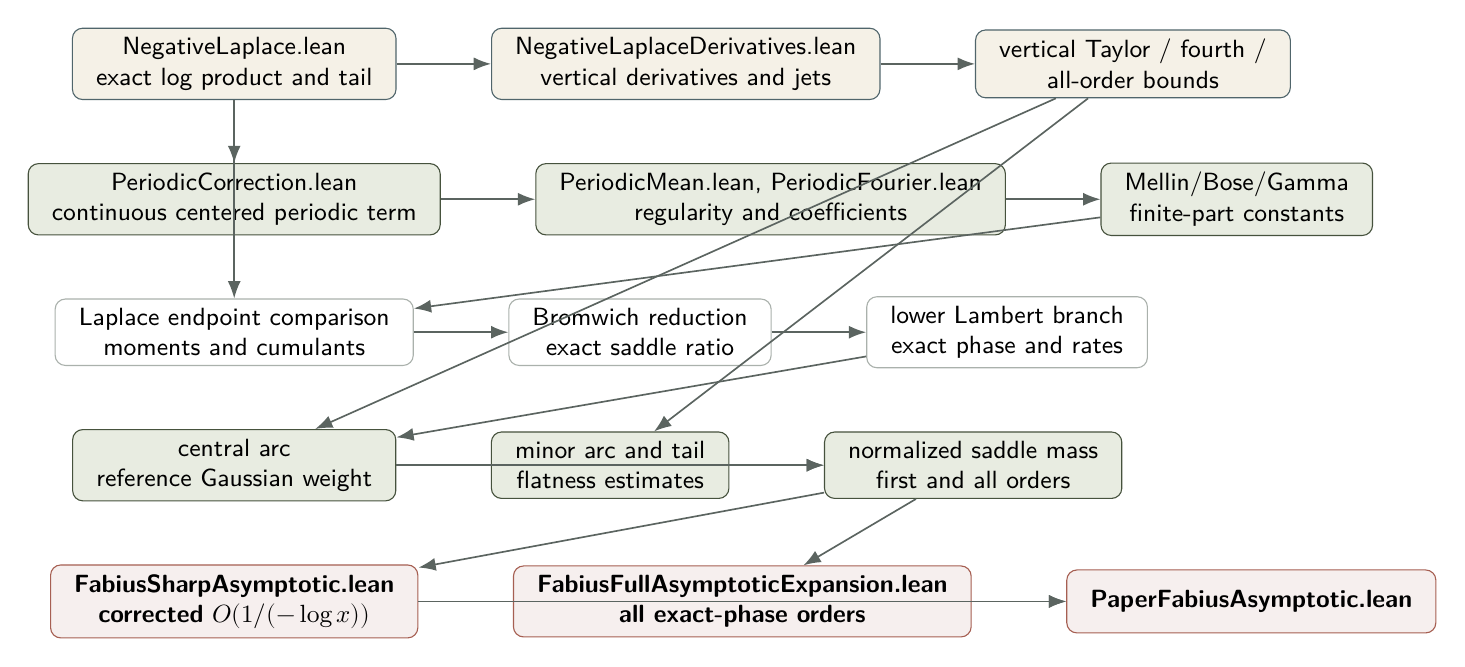
\begin{tikzpicture}[node distance=8mm and 12mm]
  \node[mathmod] (neg) {\module{NegativeLaplace}\\exact log product and tail};
  \node[mathmod,right=of neg] (der) {\module{NegativeLaplaceDerivatives}\\vertical derivatives and jets};
  \node[mathmod,right=of der] (vbound) {vertical Taylor / fourth /\\all-order bounds};

  \node[mod,below=of neg] (per) {\module{PeriodicCorrection}\\continuous centered periodic term};
  \node[mod,right=of per] (preg) {\module{PeriodicMean}, \module{PeriodicFourier}\\regularity and coefficients};
  \node[mod,right=of preg] (mellin) {Mellin/Bose/Gamma\\finite-part constants};

  \node[generic,below=of per] (lap) {Laplace endpoint comparison\\moments and cumulants};
  \node[generic,right=of lap] (brom) {Bromwich reduction\\exact saddle ratio};
  \node[generic,right=of brom] (lam) {lower Lambert branch\\exact phase and rates};

  \node[mod,below=of lap] (central) {central arc\\reference Gaussian weight};
  \node[mod,right=of central] (tail) {minor arc and tail\\flatness estimates};
  \node[mod,right=of tail] (mass) {normalized saddle mass\\first and all orders};

  \node[facade,below=of central] (sharp) {\module{FabiusSharpAsymptotic}\\corrected $O(1/(-\log x))$};
  \node[facade,right=of sharp] (full) {\module{FabiusFullAsymptoticExpansion}\\all exact-phase orders};
  \node[facade,right=of full] (paper) {\module{PaperFabiusAsymptotic}};

  \draw[arrow] (neg)--(der);
  \draw[arrow] (der)--(vbound);
  \draw[arrow] (neg)--(per);
  \draw[arrow] (per)--(preg);
  \draw[arrow] (preg)--(mellin);
  \draw[arrow] (neg)--(lap);
  \draw[arrow] (mellin)--(lap);
  \draw[arrow] (lap)--(brom);
  \draw[arrow] (brom)--(lam);
  \draw[arrow] (vbound)--(central);
  \draw[arrow] (lam)--(central);
  \draw[arrow] (vbound)--(tail);
  \draw[arrow] (central)--(mass);
  \draw[arrow] (tail)--(mass);
  \draw[arrow] (mass)--(sharp);
  \draw[arrow] (mass)--(full);
  \draw[arrow] (sharp)--(paper);
  \draw[arrow] (full)--(paper);
\end{tikzpicture}}
\caption{The corrected asymptotic tower.  Several boxes stand for families of
small modules; the direction is exact algebra $\to$ regularization $\to$
quantitative saddle estimates $\to$ source-facing theorems.}
\label{fig:asymptotic-dag}
\end{figure}

\section{Why there are many small asymptotic modules}
A saddle proof contains qualitatively different tasks: exact identities,
complex differentiability, local Taylor bounds, Gaussian moment algebra,
minor-arc decay, phase selection, and asymptotic transfer between variables.
Putting all of them in one file would make imports cyclic and theorem statements
unreadable.  The module granularity records the proof obligations:
\begin{description}
\item[\module{NegativeLaplaceVertical*}] control the complex logarithm and its
ordinary or logarithmic jets on vertical lines.
\item[\module{GaussianPolynomial*}] evaluate or bound Gaussian integrals with
polynomial corrections.
\item[\module{FabiusSaddleReference*}] define the normalized reference weight
and control its tails.
\item[\module{FabiusSaddleCentral*}] compare the true central integrand with its
finite expansion.
\item[\module{FabiusSaddleTail*}] prove the complement is negligible, first
quantitatively and then to every order.
\item[\module{SaddleExpansion*}] provide generic algebra for finite asymptotic
series, logarithms, and flat additions.
\end{description}
The final modules can then state a sharp theorem in a few lines because every
analytic estimate has a named interface.

% ================================================================================
\chapter{The periodic correction and its Mellin analysis}
\label{ch:periodic}

\section{Centering the exact periodic term}
The raw periodic correction from \module{NegativeLaplace} is initially a value
defined from convergent series at positive arguments.  \module{PeriodicCorrection}
proves local uniform convergence on compact positive intervals using explicit
Weierstrass majorants.  Continuity in $s$ transfers to continuity in
$t=\log_2s$, and the exact dilation law gives period one.

The module defines a centered function \decl{negativeLaplacePsi} by subtracting
the period mean:
\[
 \int_0^1\Psi(t)\,dt=0,
 \qquad \Psi(t+1)=\Psi(t).
\]
Centering is not just cosmetic.  It makes the constant part of the asymptotic
main term canonical and places all oscillation in a zero-mean function whose
Fourier coefficients are unambiguous.

\section{Mean, smoothness, and Fourier coefficients}
The next modules divide regularity questions by strength.
\begin{description}
\item[\module{PeriodicMean}] computes or identifies the mean and proves the
integral manipulations needed to center the correction.
\item[\module{PeriodicRegularity}] differentiates the periodized series with
uniform bounds on compact sets.
\item[\module{PeriodicSmooth}] packages $C^\infty$ regularity.
\item[\module{PeriodicFourier}] proves Fourier coefficient formulas, convergence
of the Fourier series at the needed strength, and nonconstancy consequences.
\end{description}
The separation matters because the sharp $O(1/t)$ theorem only needs bounded
regularity at certain stages, while the obstruction theorem needs a certified
nonzero oscillatory component.

\section{Mellin regularization}
The Fourier coefficients of a log-dyadic periodization naturally involve a
Mellin transform.  The zero frequency is singular and must be treated as a
finite part.  The files \module{MellinBose},
\module{BoseFinitePartIntegral}, and \module{MellinFinitePart} formalize this
without hiding the pole cancellation.

Near $s=0$, the product $\Gamma(s)\zeta(1+s)$ has a double pole.  The code
subtracts the principal part and defines a regular product whose limit is the
constant \decl{gammaZetaConstant}.  It proves both a complex punctured limit
and the real one-sided limit used in the final main term.  Auxiliary modules
\module{GammaSecondOrder} and \module{StieltjesConstant} provide the exact
second-order expansions and the chosen first Stieltjes constant convention.

\begin{engineering}
The constant is carried as a named exact expression rather than a decimal.
This prevents sign-convention mistakes for the first Stieltjes constant and
allows the compact Lambert formula to be algebraically expanded into the
literal Euler--Stieltjes form only in the dedicated Wikipedia-expansion module.
\end{engineering}

\section{The periodic term is genuinely nonconstant}
The Fourier analysis proves that at least one nonzero Fourier coefficient of
\decl{negativeLaplacePsi} is nonzero.  Therefore $\Psi$ cannot be absorbed into
the constant.  Since its phase tends to infinity while advancing through all
residue classes modulo one, it contributes bounded but persistent oscillation
to $\log F(x)$.

This is the decisive fact behind the correction.  A remainder bounded by
$C/(-\log x)$ tends to zero.  A nonconstant periodic function sampled at the
exact phase does not.  Therefore an elementary main term omitting $\Psi$ cannot
have the claimed inverse-logarithmic error.

\section{Endpoint Laplace comparison}
The transform asymptotic must eventually become a statement about the function
near its endpoint.  \module{EndpointLaplaceComparison} relates the Laplace
integral to a local endpoint mass and controls the difference.  Positivity,
monotonicity, and compact support allow upper and lower bounds that isolate the
same saddle scale.  \module{LaplaceMomentBounds} and
\module{LaplaceCumulantAsymptotics} supply derivative information and convexity
for the logarithmic transform.

This comparison is an important conceptual bridge: the product describes a
transform globally, while the theorem concerns $F(x)$ locally as $x\to0^+$.
The formalization does not silently identify the two; it proves an exact or
quantified transfer theorem and names the residual ratio.

% ================================================================================
\chapter[The lower Lambert phase and the corrected sharp asymptotic]{The lower Lambert phase and the\\corrected sharp asymptotic}
\label{ch:sharp}

\section{The exact phase equation}
The saddle coordinate is not the naive dyadic logarithm
$t=-\log_2x$.  It is the lower-Lambert solution $\lambda$ of
\[
 \lambda 2^{-\lambda}=x.
\]
Equivalently,
\[
 \lambda-\log_2\lambda=t.
\]
The file \module{LowerLambertW} constructs the lower real branch by inverting
$u\mapsto u\log u$ on the appropriate interval, proves the equation and branch
inequalities, and packages the paper's solution \decl{paperLambertN}.

For the small-argument variable,
\[
 \lambda(x)=
 -\frac{W_{-1}(-x\log2)}{\log2}.
\]
The declaration is \decl{fabiusLambertPhase}.  On the dyadic logarithmic scale,
\decl{dyadicLambertPhase t} is the same quantity at $x=2^{-t}$.
\module{FabiusLambertPhase} proves
\[
 \lambda(t)=t+\log_2t+o(1)
\]
and refines this to the quantitative remainders needed by the literal
$O(1/t)$ expansion.

\begin{proofidea}
Keeping $\lambda$ exact makes the saddle stationary by definition.  Replacing
it too early by $t+\log_2t$ shifts the phase of the periodic correction.  Even
a small absolute phase error can create an error larger than $1/t$ after a
nonconstant periodic function is composed with it.
\end{proofidea}

\section{The compact corrected main term}
The cleanest source-facing expression is defined in
\module{FabiusWikipediaMain}.  Put
\[
 W=W_{-1}(-x\log2),\qquad
 \lambda=-W/\log2.
\]
Then
\begin{align*}
 M_{\mathrm{corr}}(x)
  ={}&-\frac{7\log2}{12}-\frac12\log(\pi x)\\
    &+\frac{\gamma_\ast-W-\tfrac12W^2}{\log2}
      +\Psi(\lambda),
\end{align*}
where $\gamma_\ast$ is \pathbreak{gammaZetaConstant} and $\Psi$ denotes
\pathbreak{negativeLaplacePsi}.  In Lean the displayed expression is
\pathbreak{fabiusCorrectedWikipediaMain}.  The file proves it is exactly equal
to the internal saddle main \pathbreak{fabiusSharpLambertMain} whenever the lower
Lambert branch lies in its natural domain.

The equality uses only the exact saddle equation.  Taking logarithms of
$\lambda2^{-\lambda}=x$ gives
\[
 \log x=\log\lambda-(\log2)\lambda,
\]
which converts the transform-side exponent to the compact $W$ expression.

\section{The literal elementary expansion}
\module{FabiusWikipediaExpansion} expands the compact main into powers of
$\log x$ and $\log(-\log x)$.  It defines
\decl{fabiusWikipediaElementaryMain}, the nonperiodic expression appearing in
the source discussion, including its Euler--Stieltjes constant and the visible
$1/\log x$ correction.  The corrected literal main is
\[
 M_{\mathrm{explicit}}(x)
 =M_{\mathrm{elementary}}(x)+\Psi(\lambda(x)).
\]

On $x=2^{-t}$, its nonperiodic component is organized as
\begin{align*}
 -\frac{\log2}{2}t^2-t\log t
 &+\left(1+\frac{\log2}{2}\right)t
 -\frac{(\log t)^2}{2\log2}+C\\
 &-\frac{(\log t)^2}{2(\log2)^2t},
\end{align*}
plus an explicit source-conversion term of order $1/t$.  A fourth phase term
from \module{FabiusLambertHigherExpansion} is needed: stopping one refinement
earlier would leave $O((\log t)/t)$, not $O(1/t)$.

\section{Central arc, minor arc, and normalized mass}
The saddle proof is split into a central region and its complement.

\begin{description}
\item[Reference weight.] \module{FabiusSaddleReferenceWeight} defines the
Gaussian-normalized measure after centering at the exact saddle.  Its total
mass and polynomial moments are controlled by the \module{GaussianPolynomial*}
files.
\item[Central comparison.] \module{FabiusSaddleCentral} and
\module{FabiusSaddleCentralLambert} Taylor-expand the vertical logarithm,
exponentiate the controlled remainder, and compare the true central integrand
with the reference Gaussian weight.
\item[Minor arc and tail.] \module{NegativeLaplaceMinorArc},
\module{FabiusLambertMinorArc}, \module{FabiusSaddleTail}, and reference-tail
modules show that away from the saddle the real part drops uniformly.  The
tail is small at the quantitative order needed for the sharp theorem.
\item[Exact reduction.] \module{FabiusSharpExactReduction} expresses
$\log F(x)-M_{\mathrm{corr}}(x)$ as the logarithm of a normalized saddle ratio
plus the exponentially small forward-tail error.
\end{description}

The headline analytic estimate is that the normalized saddle kernel mass is
$1+O(1/\lambda)$.  Taking a logarithm preserves the order because the ratio is
eventually positive and tends to one.

\section{The corrected theorem and the obstruction theorem}
\module{FabiusSharpAsymptotic} exposes three complementary statements.  For
any \code{F} satisfying \decl{IsFabius},
\[
 \log F(x)-M_{\mathrm{explicit}}(x)
   =O\!\left(\frac1{-\log x}\right)
 \qquad(x\to0^+).
\]
This is
\decl{log_fabius_sub_explicitCorrectedWikipediaMain_isBigO}.  The compact
Lambert form has an analogous theorem.

The file also proves the negative statement
\[
 \log F(x)-M_{\mathrm{elementary}}(x)
 \ne O\!\left(\frac1{-\log x}\right),
\]
through \decl{log_fabius_sub_WikipediaElementaryMain_not_isBigO}.  The proof
uses nonconstancy of $\Psi$ and sequences of exact phases approaching two
points with different periodic values.  Thus the missing term is not optional
at the claimed precision.

Finally, exponentiating a logarithmic error tending to zero gives
\[
 F(x)\sim \exp(M_{\mathrm{explicit}}(x)).
\]
Lean proves this by rewriting the quotient as the exponential of the log
difference, using strict positivity of $F(x)$ for $x>0$, and composing the
error limit with continuity of \code{Real.exp}.

\begin{correction}
The formal result is stronger than replacing a wrong constant.  It identifies
a missing \emph{nonconstant periodic function}, fixes the phase at the exact
lower-Lambert coordinate, proves the repaired inverse-logarithmic error, and
proves that the uncorrected claim fails at that same rate.
\end{correction}

\section{Why a quotient-of-exponentials fit is not an asymptotic equivalent}
\module{FabiusQuotientExponentialMismatch} analyzes a visually effective
compact-interval fit built from a quotient of exponentials.  Its endpoint decay
is of $e^{-c/x}$ type.  The Fabius function decays faster than every power but
slower than $e^{-c/x}$ for every fixed $c>0$.  Therefore the quotient fit tends
to zero too rapidly and cannot be an asymptotic equivalent, even if it is
numerically attractive away from the endpoint.

The qualitative comparison is formalized separately in
\module{FabiusFlatness} and \module{FabiusDecayComparison}; the mismatch module
then turns those rates into a quotient or non-equivalence theorem.

% ================================================================================
\chapter{The full exact-phase asymptotic expansion}
\label{ch:all-orders}

\section{A generic notion of expansion}
The all-orders branch does not encode each truncation as an unrelated theorem.
The \module{SaddleExpansion*} files define a reusable
\decl{HasAsymptoticExpansion} interface.  Given a filter $\mathcal F$, a small
scale $\varepsilon(x)$, a target $f(x)$, and coefficient functions $a_j(x)$,
the structure records:
\begin{itemize}
  \item every coefficient term has the expected Big-$O$ size;
  \item for every $N$, the difference between $f$ and
        $\sum_{j<N}\varepsilon^j a_j$ is $O(\varepsilon^N)$.
\end{itemize}
The coefficients are permitted to depend on $x$.  This is essential here:
they are periodic functions evaluated at the exact Lambert phase, not fixed
constants.

The generic library proves closure under finite sums, products, scalar
operations, addition of a flat function, and composition with a logarithm near
one.  Separate algebra modules handle coefficient convolution and the formal
logarithm recurrence.

\section{Vertical jets and finite exponential algebra}
The complex saddle exponent is Taylor-expanded in the vertical variable.  The
modules
\begin{itemize}
  \item \module{NegativeLaplaceVerticalOrdinaryJets},
  \item \module{NegativeLaplaceAllOrderJets},
  \item \module{NegativeLaplaceVerticalAllOrderBound}, and
  \item \module{FabiusSaddleExponentAllOrders}
\end{itemize}
provide an arbitrary finite jet together with a uniform remainder on the
central arc.

Exponentiating a truncated polynomial produces coefficients indexed by
partitions of the total order.  Rather than asking ring normalization to
rediscover this combinatorics in every theorem, \module{SaddleExpansionAlgebra},
\module{SaddleExpansionFiniteRemainder}, and
\module{FabiusSaddlePolynomialCoefficients} define the coefficient recursion
and prove the finite remainder estimate abstractly.

\section{Gaussian contraction of polynomial corrections}
After scaling, odd Gaussian moments vanish and even moments are explicit.  The
files \module{GaussianPolynomialContraction},
\module{GaussianPolynomialWholeIntegral},
\module{GaussianPolynomialTail}, and
\module{GaussianPolynomialTailAllOrders} convert the exponent coefficients
into mass coefficients.  They also prove that replacing a finite central
interval by the whole Gaussian line produces an error flat to every requested
order once the central radius grows appropriately.

The output is \decl{fabiusSaddleMassCoefficient j lam}, a real coefficient
function of the exact phase $\lambda$.  Its dependence on $\lambda$ contains
the periodic derivative data inherited from the negative Laplace correction.
The zeroth coefficient is one.

\section{Central and tail estimates to every order}
\module{FabiusSaddleCentralAllOrders} proves that the central kernel mass has
the finite expansion with a remainder of order $\lambda^{-N}$.
\module{FabiusSaddleTailAllOrders} proves that the omitted saddle contour is
flat compared with every such power.  \module{FabiusSaddleMassAllOrders} adds
the pieces and packages a single expansion theorem.

The distinction between “central remainder” and “tail flatness” is important.
The central error is produced by truncating an analytic Taylor series and must
be tracked at exactly order $N$.  The tail is exponentially or superpolynomially
small and can be added through a generic \decl{add_flat} theorem without
changing any coefficient.

\section{From complex kernel mass to a real saddle ratio}
The kernel analysis is naturally complex, but the Fabius saddle ratio is real.
\module{FabiusFullAsymptoticExpansion} first proves that complexification of the
real ratio equals the kernel mass.  Norm compatibility then transfers both
coefficient and remainder estimates:

\begin{LeanCode}
theorem fabiusSaddleRatio_dyadicLambert_hasAsymptoticExpansion
    (F : BoundedFabius) (hF : IsFabius F) :
    HasAsymptoticExpansion atTop
      (fun t : ℝ => (dyadicLambertPhase t)⁻¹)
      (fun t : ℝ => fabiusSaddleRatio F ((2 : ℝ) ^ (-t))
        (fabiusLambertRadius ((2 : ℝ) ^ (-t)))
        (dyadicLambertPhase t))
      (fun j t =>
        fabiusSaddleMassCoefficient j (dyadicLambertPhase t)) := by
  ...
\end{LeanCode}

This theorem is the all-orders analogue of the first-order statement that the
normalized mass equals $1+O(1/\lambda)$.

\section{Taking the logarithm}
The desired expansion is for $\log F$, so the ratio expansion must pass through
\code{Real.log}.  The generic method \decl{HasAsymptoticExpansion.real_log}
requires:
\begin{itemize}
  \item the small scale tends to zero;
  \item the zeroth mass coefficient is identically one;
  \item the target ratio is eventually positive.
\end{itemize}
All three are proved explicitly.  The logarithmic coefficient recurrence is
packaged as \pathbreak{fabiusSaddleLogCoefficient}.  The zeroth log coefficient
vanishes, as it should for the logarithm of a series beginning with one.

The exponentially flat forward-tail error from \module{NegativeLaplace} is
then added with the generic flat-addition theorem.  This is a particularly clean
payoff of the exact decomposition: the forward tail never enters the coefficient
recursion.

\section{Finite truncations and the first explicit correction}
Define
\[
 S_N(\lambda)=\sum_{j=0}^{N-1}
 \lambda^{-j}c_j(\lambda)
\]
after logarithmic coefficient conversion, and
\[
 M_N(x)=M_{\mathrm{sharp}}(x)+S_N(\lambda(x)).
\]
These are \decl{fabiusSaddleLogPartialSum} and
\decl{fabiusSharpLambertExpansion}.  For every $N$,
\[
 \log F(x)-M_N(x)=O(\lambda(x)^{-N}).
\]
Since $\lambda(x)$ is comparable to $-\log x$, the file also exports the weaker
but more elementary rate
\[
 O\bigl(({-\log x})^{-N}\bigr).
\]

At $N=2$, the zeroth term vanishes and the first correction is explicit:
\[
 S_2(\lambda)=
 \frac{\operatorname{fabiusFirstSaddleCorrection}(\lambda)}{\lambda}.
\]
The coefficient is periodic/phase-dependent; the theorem identifies it but
does not assert it is nowhere zero.

\section{Transport from the dyadic logarithmic scale to \texorpdfstring{$x\to0^+$}{x to 0+}}
Most quantitative work is done with $x=2^{-t}$ and $t\to+\infty$, where dyadic
periodicity and the Lambert phase are natural.  The generic module
\module{SaddleExpansionSmallArgument} proves a filter-transfer theorem between
these coordinates.  \module{SaddleLogAsymptoticTransfer} handles the logarithmic
form and scale comparison.  The final theorem is:

\begin{LeanCode}
theorem log_fabius_sub_sharpLambertMain_hasAsymptoticExpansion
    (F : BoundedFabius) (hF : IsFabius F) :
    HasAsymptoticExpansion (nhdsWithin 0 (Set.Ioi 0))
      (fun x : ℝ => (fabiusLambertPhase x)⁻¹)
      (fun x : ℝ => Real.log (fabiusReal F x) -
        fabiusSharpLambertMain x)
      (fun j x => fabiusSaddleLogCoefficient j
        (fabiusLambertPhase x)) := by
  ...
\end{LeanCode}

The finite-sum corollary
\decl{log_fabius_sub_sharpLambertExpansion_isBigO} is usually the most convenient
consumer API.

\section{What is and is not expanded}
The phase itself is developed to arbitrary order in
\module{FabiusLambertAllOrderAlgebra},
\module{FabiusLambertAllOrderRemainder},
\module{FabiusLambertAllOrderSmallArgument}, and related higher-expansion
modules.  Nevertheless the final saddle coefficients remain evaluated at the
\emph{exact} phase $\lambda(x)$.

Substituting an asymptotic expansion for $\lambda$ inside every oscillatory
coefficient $c_j(\lambda)$ is a separate composition problem.  One would need
all-order Taylor control of periodic coefficient functions and careful
bookkeeping of phase perturbations.  The source comments explicitly decline to
claim that additional theorem.  This is mathematical precision, not an
unfinished proof: the exact-phase expansion is already a full expansion at
all orders in $1/\lambda$.

\begin{engineering}
The all-orders theorem is parameterized by coefficient functions rather than a
single formal series with constant coefficients.  That design exactly matches
log-periodic asymptotics.  Forcing constant coefficients would either lose the
oscillation or bury it in a nonstandard generalized coefficient ring.
\end{engineering}

\section{Dyadic and \texorpdfstring{$q$-binomial}{q-binomial} sharp transfers}
A parallel family—\module{DyadicSharpDecomposition},
\module{DyadicSharpConditional}, \module{FabiusDyadicSharpCumulant},
\module{FabiusDyadicSharpAsymptotic}, and the $q$-binomial sharp-transfer
modules—specializes the small-argument theory to exact dyadic sequences or
finite formulas.  The strategy is to insert an exact dyadic representation
before taking the asymptotic limit.  This permits statements about exact
rational sequences whose logarithms inherit the same Lambert/periodic behavior.

The conditional files separate a generic asymptotic implication from the
specific analytic estimates needed to discharge it.  That structure makes it
possible to experiment with alternate discrete decompositions without
rebuilding the saddle proof.

% ================================================================================
\chapter{Recurring Lean proof-engineering patterns}
\label{ch:engineering}

\section{Carry invariants in types when they are truly structural}
\decl{BoundedFabius} stores the range $[0,1]$ in the codomain.  The fixed-point
space stores symmetry as a subtype condition.  Probability coordinates use
\code{Set.Icc 0 1}.  These choices move ubiquitous obligations from theorem
hypotheses into projections from the type.

The project does not apply this maxim indiscriminately.  Compact support, for
example, remains a proposition rather than a bespoke function type because it
is proved for several derived functions and consumed by standard mathlib APIs.
The practical rule is: put an invariant in the type when almost every operation
must preserve it and there is a natural complete/algebraic structure on the
subtype.

\section{Prove exact algebra before casting}
Moment recurrences, Thue--Morse sums, $q$-binomial identities, and dyadic values
are proved over $\N$, $\Z$, or $\Q$.  Cast the final theorem to $\R$ or $\C$.
This preserves decidable equality, normalization, parity, divisibility, and
kernel computation.  The bridge lemmas are then explicit and searchable,
usually with names ending in \code{_cast}.

\section{Separate implementation invariants from mathematical specifications}
The dyadic evaluator is the clearest example:
\begin{itemize}
  \item table length, prefix stability, and recursion decrease are program
        properties;
  \item block Taylor and bit recurrence are mathematical properties;
  \item a generic strong-induction theorem connects them.
\end{itemize}
This makes refactoring possible.  A vector-backed or memoized table could reuse
the mathematical recurrence after reproving only the implementation interface.

\section{Use local finiteness instead of unnecessary convergence theory}
The signed global extension is written as a \code{tsum}, but every local proof
reduces it to a finite sum by support.  The same principle appears in
partitions of unity and translated bump sums.  When a series is locally finite,
proving absolute convergence of every derivative is both harder and less
informative than proving a local finite support set.

\section{Package smooth compact support as Schwartz only at transform boundaries}
The code does not make \upfun a Schwartz map at its definition site.  It first
proves smoothness and support in ordinary function language.  Modules that need
Fourier injectivity or Poisson summation then package those facts into a
Schwartz object.  This avoids forcing all elementary lemmas through coercions
from a heavyweight bundled type.

\section{Strong induction follows binary control flow}
Binary algorithms often recurse neither on the scale alone nor on the immediate
predecessor.  Clearing the highest set bit produces an arbitrary smaller
natural.  \code{Nat.strong_induction_on} matches the program and avoids
inventing an artificial measure.  The same style appears in coefficient
uniqueness arguments where the $n$th coefficient depends on all earlier ones.

\section{Use formal power series for coefficient identities}
Analytic power-series proofs carry convergence radii and topology even when the
claim is purely finite coefficient algebra.  The moment and $q$-binomial
branches use formal series until a theorem genuinely needs evaluation at a real
or complex argument.  Coefficient extraction then turns multiplication into a
finite convolution with no summability side conditions.

\section{Normalize before proving parity or divisibility}
A rational recurrence obscures parity.  Clearing a carefully chosen common
denominator creates a natural recurrence where “all terms but one are even” is
visible to \code{omega}, \code{norm_num}, and divisibility lemmas.  The normalized
sequence is not auxiliary clutter; it is the correct domain for the theorem.

\section{Factor generic convergence arguments away from special coefficients}
The interval-average squeezing theorem, finite-row Toeplitz theorem, generic
Legendre convergence theorem, generic least-squares projection theorem, and
generic saddle-expansion algebra all follow this pattern.  The special branch
proves a small interface—monotonicity, bounded variation, smoothness, or a
finite jet—and the generic theorem handles the limiting logic.

\section{Prefer exact cancellation to estimation when symmetry allows it}
Taylor reduction cancels two remainders rather than bounding them.  Complete
Thue--Morse blocks annihilate low-degree polynomials exactly.  Odd Legendre
coefficients vanish exactly.  The negative-Laplace dilation equation is solved
with an exact periodic correction before the remaining tail is estimated.
Exact symmetry usually yields stronger theorems and simpler downstream error
bookkeeping.

\section{Make false source claims first-class}
The repository uses counterexample and obstruction modules instead of merely
editing comments.  A negative theorem such as
\decl{log_fabius_sub_WikipediaElementaryMain_not_isBigO} is a durable API: later
work cannot accidentally assume the discarded statement, and a reader can see
precisely which quantifier or rate fails.

\section{Control coercions at named boundaries}
Common coercion seams include:
\begin{itemize}
  \item subtype value $\to\R$ through \decl{fabiusReal};
  \item $\Q\to\R$ through exact \code{_cast} theorems;
  \item real functions $\to$ complex functions for Fourier/Laplace analysis;
  \item real ratios $\to\C$ kernel masses in the saddle proof;
  \item natural floor lengths $\leftrightarrow$ integer floor endpoints in
        discrete sums.
\end{itemize}
Each seam receives a lemma.  This is preferable to repeated local
\code{norm_cast} improvisation, which tends to make proofs brittle under
normal-form changes.

\section{Keep endpoint facts explicit}
Many informal proofs say “the boundary term vanishes.”  Here the reason may be
constant tails, compact support, flatness at zero, flatness at a power of two,
or the factor $1-x^2$ in the Legendre operator.  The code records each as a
separate theorem and invokes exactly the right one in integration by parts or
gluing.  This makes corrections to endpoint conventions local.

% ================================================================================
\chapter{Task-oriented reading paths and extension points}
\label{ch:reading}

\section{To understand the canonical construction}
\begin{readingpath}
Read \module{Basic}, the first half of \module{Differential}, and then
\module{Existence}.  Keep mathlib documentation for complete metric spaces,
continuous maps on compact sets, Bochner/interval integrals, and contraction
maps nearby.  After the fixed point is built, return to the smoothness
bootstrap in \module{Differential} and finally read the uniqueness tail of
\module{Existence}.
\end{readingpath}
The main extension point is an alternative construction: prove the resulting
object satisfies \decl{IsFabius}; the uniqueness API supplies equality with the
canonical function.

\section{To modify or optimize the dyadic evaluator}
\begin{readingpath}
Read \module{Arithmetic}'s evaluator definitions, then all of
\module{DyadicCorrectness}.  Treat \decl{FabiusDyadicHasBitRecurrence} as the
semantic interface.  Read \module{DyadicClosedForm} only after understanding
which recurrence the implementation needs, and \module{DyadicAnalytic} last.
\end{readingpath}
A performance refactor should preserve the public exact functions or provide
conversion theorems.  Likely reusable pieces are table-prefix stability,
representation refinement, and the strong-induction correctness theorem.

\section{To add a new exact arithmetic theorem}
Start from \module{MomentPowerSeries}, \module{NormalizedMoments}, and
\module{Arithmetic}.  Decide first whether the claim belongs to $\Q$,
normalizing naturals, or a real cast.  Prove the strongest exact statement in
the smallest type, then add a cast theorem near the existing analytic bridge.
For parity or valuation, introduce a division-free normalization before
attempting induction.

\section{To follow the first paper}
Read \module{Paper05442} with the paper open, jumping to:
\begin{itemize}
  \item \module{OriginalCharacterization} and \module{OriginalUniqueness} for
        Theorem 1;
  \item \module{EarlyApproximants}, \module{StepApproximationLimit}, and
        \module{WeakConvergence} for the finite approximants;
  \item \module{ProbabilityRepresentation} for the random-series model;
  \item \module{AnalyticMoments} and \module{FourierProduct} for moments and
        transform;
  \item \module{PoissonSummation} for lattice identities.
\end{itemize}
Read \module{OriginalPaperSupplement} whenever a displayed equation is not
represented by a numbered theorem in the facade.

\section{To follow the arithmetic paper}
Read \module{Paper06487} for the numbered map, then
\module{Paper06487Supplement}.  The mechanism-oriented path is
\begin{center}
\module{GlobalExtension} $\longrightarrow$
\module{ScaleTranslation} $\longrightarrow$
\module{TaylorReduction} $\longrightarrow$
\module{GlobalDyadic} $\longrightarrow$
\module{DenominatorBound} $\longrightarrow$
\module{TwoAdic}.
\end{center}
For exact inverse powers, detour through \module{MomentPowerSeries} and
\module{AnalyticMoments}.

\section{To work on \texorpdfstring{$q$-binomial}{q-binomial} or discrete formulas}
Begin with \module{HalfQBinomial} and the \module{ThueMorse*} modules.  Then
read the raw $q$-binomial formula before the simplified facade.  For limits,
read \module{FabiusDiscreteLimitToeplitz}; its generic theorem tells you the
three properties a new outer row must satisfy.  The spline module is the best
worked example of binary block cancellation with a floor-defined prefix.

\section{To work on spectral approximation}
Read \module{LegendrePolynomial} and
\module{LegendreSeriesConvergence} without Fabius context first.  Then
\module{FabiusLegendreCoefficients} shows how exact moments enter.  Finally
read \module{FabiusLegendreSeries} and
\module{FabiusLegendreLeastSquares}.  A new orthogonal basis should follow the
same pattern: generic convergence/orthogonality below, exact Fabius coefficient
bridge above.

\section{To work on the asymptotic theory}
\begin{readingpath}
Do not start with \module{FabiusSharpAsymptotic}.  Read
\module{NegativeLaplace}, \module{PeriodicCorrection}, and
\module{FabiusWikipediaMain} first.  Then study
\module{FabiusSharpExactReduction} to see the exact identity that the saddle
estimate must close.  For first order, follow the central/tail Lambert modules.
For all orders, learn the generic \module{SaddleExpansion*} API before reading
\module{FabiusSaddleMassAllOrders} and
\module{FabiusFullAsymptoticExpansion}.
\end{readingpath}
A new refinement should preserve the exact phase until the final transfer.  If
substituting an elementary phase expansion inside periodic coefficients, state
and prove a composition theorem rather than relying on informal smoothness.

\section{Where to place a new theorem}
A practical placement rule is:
\begin{description}
\item[Generic mathematical lemma] goes in the lowest module with no unnecessary
Fabius imports.
\item[Fabius bridge between two established models] gets its own focused module
or joins the existing bridge module.
\item[Exact executable or rational identity] belongs below analytic casts.
\item[Paper-numbered restatement] belongs in the relevant facade after the
mechanism theorem exists.
\item[Correction or refutation] should be named explicitly and documented in
an audit/supplement module, not hidden in a changed formula.
\end{description}

\appendix
\chapter{Categorized module catalogue}
\label{app:catalogue}
This appendix lists every module under \pathbreak{Lean/FabiusFunction/} at the pinned snapshot.  The descriptions state the module's architectural role, not an exhaustive inventory of declarations.  The root umbrella \pathbreak{Lean/FabiusFunction.lean} is listed separately after the table.
\renewcommand{\arraystretch}{1.08}
\begin{longtable}{@{}>{\raggedright\arraybackslash}p{.28\textwidth}p{.65\textwidth}@{}}
\toprule
Module & Principal role \\
\midrule
\endfirsthead
\toprule
Module & Principal role (continued) \\
\midrule
\endhead
\midrule
\multicolumn{2}{r}{\small Continued on next page} \\
\endfoot
\bottomrule
\endlastfoot
\multicolumn{2}{@{}l}{\sffamily\bfseries\color{OliveDark} Core specifications, construction, and global calculus} \\
\addlinespace[.45em]
\module{Arithmetic} & Exact natural/rational definitions: moments, Thue--Morse signs, dyadic closed forms, evaluator tables, and denominator data. \\
\addlinespace[.28em]
\module{Basic} & Core types and predicates, Rvachev folding, signed extension, sinc, and transform-level vocabulary. \\
\addlinespace[.28em]
\module{Differential} & Global derivative refinement for the up function and the generic smoothness bootstrap. \\
\addlinespace[.28em]
\module{Existence} & Complete symmetric function space, contraction operator, canonical fixed point, and dyadic-density uniqueness. \\
\addlinespace[.28em]
\module{GlobalExtension} & Local finiteness, smoothness, agreement on the unit interval, and the global equation F'(x)=2F(2x). \\
\addlinespace[.28em]
\module{GlobalDyadic} & Exact rational evaluation of the signed global extension on arbitrary dyadic blocks. \\
\addlinespace[.28em]
\module{Parity} & Reusable even/odd identities for functions, coefficients, finite sums, and dyadic decompositions. \\
\addlinespace[.28em]
\module{PaperStatements} & Stable canonical declarations and paper-facing core statements shared by aggregate modules. \\
\addlinespace[.28em]
\multicolumn{2}{@{}l}{\sffamily\bfseries\color{OliveDark} Moments, recurrences, generating functions, and transforms} \\
\addlinespace[.45em]
\module{AnalyticMoments} & Integral moments of the up function, normalization, integration-by-parts recurrences, and generating identities. \\
\addlinespace[.28em]
\module{MomentPowerSeries} & Purely formal power-series recurrences and coefficient uniqueness for moments and half moments. \\
\addlinespace[.28em]
\module{NormalizedMoments} & Natural numerator and common-denominator normalization for the half-moment sequence. \\
\addlinespace[.28em]
\module{NormalizedEvenMoments} & Exact normalization and integrality properties for the even moment sequence. \\
\addlinespace[.28em]
\module{HalfMomentDenominator} & Sharper denominator products and divisibility facts for half moments. \\
\addlinespace[.28em]
\module{BernoulliRecurrences} & Bernoulli-number forms of the moment and inverse-power recurrences. \\
\addlinespace[.28em]
\module{FabiusRecurrenceSequence} & The normalized inverse-power sequence, positivity, rapid decay, recurrences, and generating series. \\
\addlinespace[.28em]
\module{ExactInversePower} & Exact formulas identifying inverse-power Fabius values with normalized moment data. \\
\addlinespace[.28em]
\module{FourierAnalytic} & Analytic/entire properties of sinc products and transform series. \\
\addlinespace[.28em]
\module{FourierProduct} & Convergence of the infinite sinc product and equality with the Fourier transform of the up function. \\
\addlinespace[.28em]
\module{LaplaceTransform} & Laplace transform definitions and identities for the canonical compactly supported density. \\
\addlinespace[.28em]
\module{LaplaceMoments} & Moment expansions and differentiation formulas for the Laplace transform. \\
\addlinespace[.28em]
\module{LaplaceMomentBounds} & Uniform bounds for Laplace moments and derivatives used in saddle estimates. \\
\addlinespace[.28em]
\module{FabiusComplexMGF} & Complex moment-generating function and analytic continuation interfaces. \\
\addlinespace[.28em]
\multicolumn{2}{@{}l}{\sffamily\bfseries\color{OliveDark} Certified dyadic evaluation, denominators, and valuations} \\
\addlinespace[.45em]
\module{DyadicCorrectness} & Program invariants and the abstract bit-recurrence theorem certifying the executable evaluator. \\
\addlinespace[.28em]
\module{DyadicClosedForm} & Thue--Morse block cancellation, polynomial/Hasse-derivative identities, and exact bit recurrence. \\
\addlinespace[.28em]
\module{DyadicAnalytic} & Analytic Taylor-block recurrence and cast equality between exact dyadic values and every Fabius solution. \\
\addlinespace[.28em]
\module{DenominatorBound} & Explicit common denominators, integrality after scaling, and LCM bounds for finite dyadic grids. \\
\addlinespace[.28em]
\module{TwoAdic} & Odd normalized numerators and exact 2-adic valuations of inverse-dyadic values. \\
\addlinespace[.28em]
\module{FabiusInverseDyadicClosedForm} & Consolidated inverse-dyadic closed formulas in final source-facing notation. \\
\addlinespace[.28em]
\module{FabiusDyadicLogBounds} & Quantitative logarithmic bounds for exact dyadic values, used in asymptotic comparison. \\
\addlinespace[.28em]
\multicolumn{2}{@{}l}{\sffamily\bfseries\color{OliveDark} Original-paper construction, probability, and approximation} \\
\addlinespace[.45em]
\module{OriginalCharacterization} & The compact-support specification with unknown scale and derivation that the scale equals two. \\
\addlinespace[.28em]
\module{OriginalUniqueness} & Schwartz packaging, Fourier refinement, infinite sinc product, and transform-injectivity uniqueness. \\
\addlinespace[.28em]
\module{OriginalPaperSupplement} & Unnumbered displayed equations, endpoint details, and corrections supporting the first paper. \\
\addlinespace[.28em]
\module{EarlyApproximants} & Finite convolution measures, characteristic polynomials, and half-endpoint step approximants. \\
\addlinespace[.28em]
\module{EarlyMeasureBridge} & Links between finite algebraic approximants and their probability-measure realizations. \\
\addlinespace[.28em]
\module{StepMeasureBridge} & Identifies step functions with densities or interval masses of the finite measures. \\
\addlinespace[.28em]
\module{StepApproximationLimit} & Unimodality, interval-average squeezing, and pointwise convergence to the up function. \\
\addlinespace[.28em]
\module{WeakConvergence} & Characteristic-function convergence and Levy continuity for the finite probability measures. \\
\addlinespace[.28em]
\module{ProbabilityRepresentation} & Infinite product probability space, weighted random series, self-similar law, and CDF identification. \\
\addlinespace[.28em]
\module{PoissonSummation} & Schwartz rapid decay of every real-axis Fourier derivative, Poisson summation, partitions of unity, period-two expansions, and source corrections. \\
\addlinespace[.28em]
\multicolumn{2}{@{}l}{\sffamily\bfseries\color{OliveDark} Translation, Taylor reduction, and arithmetic-paper support} \\
\addlinespace[.45em]
\module{ScaleTranslation} & Power-of-two translations, Thue--Morse sign flips, derivative translation, and remainder cancellation. \\
\addlinespace[.28em]
\module{TaylorReduction} & Exact finite Taylor reduction across dyadic annuli, including integer-scale branches. \\
\addlinespace[.28em]
\module{Paper06487Supplement} & Unnumbered arithmetic-paper claims, monotonicity, flatness, expanded formulas, and repaired proof factors. \\
\addlinespace[.28em]
\multicolumn{2}{@{}l}{\sffamily\bfseries\color{OliveDark} Thue--Morse, q-binomial formulas, and discrete limits} \\
\addlinespace[.45em]
\module{HalfQBinomial} & Gaussian binomial coefficients at q=1/2, finite Pochhammer products, positivity, and the finite q-binomial theorem. \\
\addlinespace[.28em]
\module{ThueMorsePrefix} & Finite signed prefixes, binary block decompositions, and iterated prefix operations. \\
\addlinespace[.28em]
\module{ThueMorseGenerating} & Formal and polynomial generating identities for signed Thue--Morse data. \\
\addlinespace[.28em]
\module{ThueMorseExponential} & Finite exponential product factorization and consequences for power-sum cancellation. \\
\addlinespace[.28em]
\module{ThueMorseApproximation} & Corrected finite approximation theorem and quantitative error estimates. \\
\addlinespace[.28em]
\module{ThueMorseBinomialLog} & Zero--one Thue--Morse sequence, binomial parity, and exact Log2 formulas. \\
\addlinespace[.28em]
\module{DraftCounterexamples} & Machine-checked counterexamples to false normalizations and error claims in the local K-fold draft. \\
\addlinespace[.28em]
\module{FabiusParityPowerSeries} & Parity-filtered formal series used to isolate even/odd Fabius coefficients. \\
\addlinespace[.28em]
\module{FabiusRawQBinomialFormula} & Unrearranged exact finite q-binomial/Thue--Morse formula close to direct expansion. \\
\addlinespace[.28em]
\module{FabiusRawQBinomialScalar} & Scalar-field generalization of the raw finite formula. \\
\addlinespace[.28em]
\module{FabiusQBinomialFormula} & Coefficient-extractor proof and simplified exact formulas for inverse powers and arbitrary dyadic numerators. \\
\addlinespace[.28em]
\module{FabiusQBinomialScalarFormula} & Real/complex scalar versions of the simplified q-binomial identity. \\
\addlinespace[.28em]
\module{FabiusQBinomialTaylor} & Taylor and coefficient-isolation interpretation of the q-binomial weights. \\
\addlinespace[.28em]
\module{FabiusDyadicQBinomialScalar} & Exact dyadic specialization of the scalar q-binomial formula. \\
\addlinespace[.28em]
\module{FabiusGlobalQBinomialSeries} & Global signed-series forms and translation consequences of the q-binomial identity. \\
\addlinespace[.28em]
\module{FabiusBinaryReductionSeries} & Binary-block reduction of global formulas into convergent or finite series. \\
\addlinespace[.28em]
\module{FabiusDiscreteLimitIntegration} & Integral and inner-prefix limits underlying the discrete approximation formula. \\
\addlinespace[.28em]
\module{FabiusDiscreteLimitComplexShift} & Real and complex translation parameters in the inner Thue--Morse polynomial limit. \\
\addlinespace[.28em]
\module{FabiusDiscreteLimitToeplitz} & Finite-row Toeplitz theorem, q-binomial row normalization, and bounded total variation. \\
\addlinespace[.28em]
\module{FabiusUniformSpline} & Half-cell-centered Thue--Morse splines, block translation, gluing, and convergence. \\
\addlinespace[.28em]
\module{FabiusComplexShiftSpline} & Complex-shift extension of the spline identities and finite polynomial cancellation. \\
\addlinespace[.28em]
\multicolumn{2}{@{}l}{\sffamily\bfseries\color{OliveDark} Legendre and polynomial approximation} \\
\addlinespace[.45em]
\module{LegendrePolynomial} & Legendre recurrence, parity, Sturm--Liouville equation, orthogonality, bounds, and normalization. \\
\addlinespace[.28em]
\module{LegendreSeriesConvergence} & Generic absolute and uniform convergence of Legendre series for smooth functions. \\
\addlinespace[.28em]
\module{FabiusLegendreCoefficients} & Exact even coefficients from moments and inverse-dyadic values; vanishing of odd coefficients. \\
\addlinespace[.28em]
\module{FabiusLegendreSeries} & Pointwise and uniform Legendre expansions of the up function with exact coefficients. \\
\addlinespace[.28em]
\module{FabiusTranslatedLegendreSeries} & Affine transport of the up-function series to the bounded Fabius function. \\
\addlinespace[.28em]
\module{FabiusLegendreLeastSquares} & Generic projection/Pythagorean theorem and the strengthened even Fabius least-squares result. \\
\addlinespace[.28em]
\multicolumn{2}{@{}l}{\sffamily\bfseries\color{OliveDark} Negative-Laplace product and vertical analytic control} \\
\addlinespace[.45em]
\module{NegativeLaplace} & Absolutely convergent logarithmic product, exact dyadic dilation law, periodic decomposition, and exponential tail. \\
\addlinespace[.28em]
\module{NegativeLaplaceDerivatives} & Derivative formulas for the negative-Laplace logarithm and termwise differentiation. \\
\addlinespace[.28em]
\module{NegativeLaplaceDerivativeBounds} & Uniform bounds for higher derivatives on positive and saddle-scale regions. \\
\addlinespace[.28em]
\module{NegativeLaplaceVertical} & Complex vertical-line evaluation near the real saddle and branch-compatible logarithms. \\
\addlinespace[.28em]
\module{NegativeLaplaceVerticalLog} & Analytic logarithm of the vertical product and exact real-axis normalization. \\
\addlinespace[.28em]
\module{NegativeLaplaceVerticalSmooth} & Smooth/holomorphic dependence of the vertical logarithm on the displacement variable. \\
\addlinespace[.28em]
\module{NegativeLaplaceVerticalTaylor} & Finite vertical Taylor formula with explicit remainder control. \\
\addlinespace[.28em]
\module{NegativeLaplaceVerticalFourthBound} & Fourth-order derivative bound used by the first quantitative saddle theorem. \\
\addlinespace[.28em]
\module{NegativeLaplaceVerticalAllOrderBound} & Arbitrary-order vertical derivative bounds for the full expansion. \\
\addlinespace[.28em]
\module{NegativeLaplaceVerticalOrdinaryJets} & Ordinary derivative jets and coefficient normalization on the vertical scale. \\
\addlinespace[.28em]
\module{NegativeLaplaceAllOrderJets} & All-order logarithmic/exponential jet package for saddle expansion. \\
\addlinespace[.28em]
\module{NegativeLaplaceMinorArc} & Decay of the product away from the central vertical neighborhood. \\
\addlinespace[.28em]
\module{NegativeLaplaceScaledTailFlat} & Superpolynomial flatness of scaled tails at the exact Lambert saddle. \\
\addlinespace[.28em]
\multicolumn{2}{@{}l}{\sffamily\bfseries\color{OliveDark} Periodic correction, Mellin finite parts, and Laplace endpoint data} \\
\addlinespace[.45em]
\module{PeriodicCorrection} & Continuity, exact period one, centering, and the zero-mean function negativeLaplacePsi. \\
\addlinespace[.28em]
\module{PeriodicMean} & Mean-value calculation and integral identities for the raw periodic correction. \\
\addlinespace[.28em]
\module{PeriodicRegularity} & Differentiability and uniform derivative convergence of the periodized series. \\
\addlinespace[.28em]
\module{PeriodicSmooth} & C-infinity packaging for the centered periodic correction. \\
\addlinespace[.28em]
\module{PeriodicFourier} & Fourier coefficients, Fourier-series representation, and nonconstancy of the periodic term. \\
\addlinespace[.28em]
\module{MellinBose} & Mellin transform of the Bose/logarithmic kernel and nonzero Fourier modes. \\
\addlinespace[.28em]
\module{MellinFinitePart} & Regularization of Gamma(s) zeta(1+s), double-pole subtraction, and the finite-part constant. \\
\addlinespace[.28em]
\module{BoseFinitePartIntegral} & Real integral representation of the finite part and endpoint justification. \\
\addlinespace[.28em]
\module{GammaSecondOrder} & Second-order expansion of the Gamma factor near zero. \\
\addlinespace[.28em]
\module{StieltjesConstant} & Chosen first Stieltjes constant convention and zeta expansion at one. \\
\addlinespace[.28em]
\module{LaplaceCumulantAsymptotics} & Large-parameter cumulant expansions and derivative scale estimates. \\
\addlinespace[.28em]
\module{LaplacePeriodicSecondOrder} & Second-order Laplace expansion retaining derivatives of the periodic correction. \\
\addlinespace[.28em]
\module{EndpointLaplaceComparison} & Quantitative transfer from transform asymptotics to endpoint values of the Fabius function. \\
\addlinespace[.28em]
\multicolumn{2}{@{}l}{\sffamily\bfseries\color{OliveDark} Lambert coordinate, saddle reduction, and sharp first-order theory} \\
\addlinespace[.45em]
\module{LowerLambertW} & Construction and uniqueness of the lower real Lambert-W branch and the equation $n2^{-n}=x$. \\
\addlinespace[.28em]
\module{FabiusLogScale} & Dyadic logarithmic coordinate and filter conversions between t to infinity and x to zero. \\
\addlinespace[.28em]
\module{FabiusSmallArgumentScale} & Common small-argument neighborhoods, positivity, and asymptotic scale comparisons. \\
\addlinespace[.28em]
\module{FabiusLogMainDefect} & Exact defect identities between logarithmic main terms and the transform-side expression. \\
\addlinespace[.28em]
\module{FabiusLambertPhase} & Exact phase lambda, fixed-point equation, two-term expansion, and quantitative remainders. \\
\addlinespace[.28em]
\module{FabiusLambertRates} & Big-O comparisons between inverse phase, inverse t, and inverse negative log x. \\
\addlinespace[.28em]
\module{FabiusLambertDerivativeBounds} & Derivative estimates for the exact phase and its refined remainders. \\
\addlinespace[.28em]
\module{FabiusLambertHigherExpansion} & Higher explicit terms needed to reach the literal O(1/t) elementary expansion. \\
\addlinespace[.28em]
\module{FabiusLambertFormalLog} & Formal logarithmic algebra for higher Lambert-phase coefficients. \\
\addlinespace[.28em]
\module{FabiusLambertSaddle} & Pairing of the exact phase with the saddle radius and stationarity identities. \\
\addlinespace[.28em]
\module{FabiusLambertMinorArc} & Minor-arc estimates expressed uniformly in the exact Lambert coordinate. \\
\addlinespace[.28em]
\module{FabiusLambertTailFlat} & All-power flatness of the forward and contour tails in inverse phase. \\
\addlinespace[.28em]
\module{BromwichSaddle} & Bromwich inversion setup, contour parameterization, and exact saddle decomposition. \\
\addlinespace[.28em]
\module{QuantitativeSaddle} & Generic central-versus-tail quantitative saddle theorem. \\
\addlinespace[.28em]
\module{FabiusBromwichInput} & Verification that the Fabius transform satisfies the generic Bromwich hypotheses. \\
\addlinespace[.28em]
\module{FabiusSaddleReduction} & Normalization of the Fabius inversion integral to a dimensionless saddle ratio. \\
\addlinespace[.28em]
\module{FabiusSaddleReferenceWeight} & Gaussian reference weight and normalization at the exact saddle. \\
\addlinespace[.28em]
\module{FabiusSaddleReferenceTail} & Tail bounds for the reference Gaussian weight. \\
\addlinespace[.28em]
\module{FabiusSaddleCentral} & Central-arc comparison with the reference weight at first quantitative order. \\
\addlinespace[.28em]
\module{FabiusSaddleCentralLambert} & First-order normalized mass estimate in the exact Lambert coordinate. \\
\addlinespace[.28em]
\module{FabiusSaddleCentralRadiusAsymptotics} & Asymptotic size and admissibility of the chosen central radius. \\
\addlinespace[.28em]
\module{FabiusSaddleTail} & First-order bound for the noncentral contour contribution. \\
\addlinespace[.28em]
\module{FabiusSharpConstant} & Exact constant assembled from Mellin, Gaussian, and scaling normalizations. \\
\addlinespace[.28em]
\module{FabiusSharpLambertMain} & Compact exact-phase logarithmic saddle main term. \\
\addlinespace[.28em]
\module{FabiusSharpLambertTransfer} & Transfer of sharp Lambert-coordinate estimates to the small-x filter. \\
\addlinespace[.28em]
\module{FabiusExplicitSharpTransfer} & Conversion from compact Lambert form to the literal log/log-log expression. \\
\addlinespace[.28em]
\module{FabiusSharpExactReduction} & Exact identity reducing log F minus the main term to log saddle ratio plus flat tail. \\
\addlinespace[.28em]
\module{FabiusSharpAsymptoticTransfer} & Generic transfer from the normalized kernel-mass estimate to the sharp theorem. \\
\addlinespace[.28em]
\module{FabiusFirstSaddleCorrection} & Closed first periodic coefficient beyond the sharp main term. \\
\addlinespace[.28em]
\module{FabiusWikipediaMain} & Corrected compact Wikipedia main term and equality with the saddle main. \\
\addlinespace[.28em]
\module{FabiusWikipediaExpansion} & Literal log x/log(-log x) expansion with exact-phase periodic correction. \\
\addlinespace[.28em]
\module{FabiusWikipediaObstruction} & Proof that omitting the nonconstant periodic correction destroys the claimed remainder. \\
\addlinespace[.28em]
\module{FabiusSharpAsymptotic} & Public corrected O(1/(-log x)) theorem, negative obstruction, and exponentiated equivalence. \\
\addlinespace[.28em]
\module{FabiusQuotientExponentialMismatch} & Endpoint-rate proof that a quotient-of-exponentials numerical fit is not asymptotically equivalent. \\
\addlinespace[.28em]
\module{FabiusFlatness} & Vanishing to every algebraic order at the endpoint and related flatness theorems. \\
\addlinespace[.28em]
\module{FabiusDecayComparison} & Faster-than-power and slower-than-exp(-c/x) comparison theorems. \\
\addlinespace[.28em]
\module{FabiusLogSquaredAsymptotic} & Coarse quadratic-log asymptotic and O(t log t) control used in the draft audit. \\
\addlinespace[.28em]
\multicolumn{2}{@{}l}{\sffamily\bfseries\color{OliveDark} All-orders saddle and Lambert expansion} \\
\addlinespace[.45em]
\module{SaddleAllOrders} & Generic all-orders saddle theorem combining finite central expansions and flat tails. \\
\addlinespace[.28em]
\module{SaddleExpansionAlgebra} & Coefficient convolution and finite asymptotic-series algebra. \\
\addlinespace[.28em]
\module{SaddleExpansionFiniteRemainder} & Remainder bookkeeping for finite products and exponentials. \\
\addlinespace[.28em]
\module{SaddleExpansionFlat} & Closure of asymptotic expansions under addition of functions flat to every order. \\
\addlinespace[.28em]
\module{SaddleExpansionSmallArgument} & Transport of expansions from logarithmic infinity to a one-sided small-argument filter. \\
\addlinespace[.28em]
\module{SaddleLogExpansionAlgebra} & Formal recurrence for logarithms of coefficient series with unit constant term. \\
\addlinespace[.28em]
\module{SaddleLogExpansionPowerSeries} & Power-series realization and coefficient correctness for the logarithmic recurrence. \\
\addlinespace[.28em]
\module{SaddleLogAsymptoticTransfer} & Generic passage from a positive ratio expansion to an expansion of its real logarithm. \\
\addlinespace[.28em]
\module{GaussianPolynomialContraction} & Finite Gaussian moment contraction of polynomial exponent coefficients. \\
\addlinespace[.28em]
\module{GaussianPolynomialWholeIntegral} & Exact whole-line Gaussian polynomial integrals. \\
\addlinespace[.28em]
\module{GaussianPolynomialTail} & Quantitative tails for Gaussian polynomial weights. \\
\addlinespace[.28em]
\module{GaussianPolynomialTailAllOrders} & Tail flatness uniformly at arbitrary asymptotic order. \\
\addlinespace[.28em]
\module{FabiusSaddlePolynomialCoefficients} & Polynomial coefficient families obtained by exponentiating the vertical jet. \\
\addlinespace[.28em]
\module{FabiusSaddleExpansionCoefficients} & Normalized mass and log coefficient definitions and structural identities. \\
\addlinespace[.28em]
\module{FabiusSaddleCoefficientRecurrence} & Finite recurrence computing successive saddle coefficients. \\
\addlinespace[.28em]
\module{FabiusSaddleExponentAllOrders} & All-order expansion of the centered complex saddle exponent. \\
\addlinespace[.28em]
\module{FabiusSaddleCentralAllOrders} & Arbitrary-order central-arc comparison and remainder. \\
\addlinespace[.28em]
\module{FabiusSaddleTailAllOrders} & Flatness of the noncentral contour contribution to every inverse-phase order. \\
\addlinespace[.28em]
\module{FabiusSaddleMassAllOrders} & Full normalized kernel-mass expansion in inverse exact Lambert phase. \\
\addlinespace[.28em]
\module{FabiusLambertAllOrderAlgebra} & Formal algebra for arbitrary-order expansion of the lower-Lambert phase. \\
\addlinespace[.28em]
\module{FabiusLambertAllOrderRemainder} & Quantitative remainder theorem for finite Lambert-phase expansions. \\
\addlinespace[.28em]
\module{FabiusLambertAllOrderSmallArgument} & Transfer of all-order phase expansions to x tending to zero. \\
\addlinespace[.28em]
\module{FabiusFullAsymptoticExpansion} & Full exact-phase expansion of $\log F$ and finite $O(\lambda^{-N})$ truncations. \\
\addlinespace[.28em]
\multicolumn{2}{@{}l}{\sffamily\bfseries\color{OliveDark} Dyadic sharp asymptotics and specialized transfers} \\
\addlinespace[.45em]
\module{DyadicSharpDecomposition} & Exact decomposition of dyadic logarithms into main, periodic, and residual terms. \\
\addlinespace[.28em]
\module{DyadicSharpConditional} & Conditional implication from discrete kernel estimates to a dyadic sharp theorem. \\
\addlinespace[.28em]
\module{FabiusDyadicSharpCumulant} & Cumulant estimates specialized to inverse-dyadic arguments. \\
\addlinespace[.28em]
\module{FabiusDyadicSharpAsymptotic} & Unconditional sharp asymptotic along exact dyadic sequences. \\
\addlinespace[.28em]
\multicolumn{2}{@{}l}{\sffamily\bfseries\color{OliveDark} Paper facades and audits} \\
\addlinespace[.45em]
\module{Paper05442} & Numbered theorem facade for arXiv:1702.05442, with explicit source corrections. \\
\addlinespace[.28em]
\module{Paper06487} & Numbered theorem facade for arXiv:1702.06487v3 and its repaired hypotheses/formulas. \\
\addlinespace[.28em]
\module{PaperFabiusAsymptotic} & Aggregate for the corrected sharp theorem, all-orders expansion, and discrete/q-binomial asymptotics. \\
\addlinespace[.28em]
\module{PaperKFoldThueMorse} & Claim-level audit of the local K-fold Thue--Morse draft, including proofs and refutations. \\
\addlinespace[.28em]
\multicolumn{2}{@{}l}{\sffamily\bfseries\color{OliveDark} Auxiliary asymptotic estimates} \\
\addlinespace[.45em]
\module{StirlingAsymptotics} & Explicit Stirling estimates and asymptotic forms used in recurrence and draft-comparison arguments. \\
\addlinespace[.28em]
\end{longtable}
\noindent\textbf{Root umbrella.}\quad \pathbreak{Analysis/FabiusFunction/Lean/FabiusFunction.lean} imports the paper facades and selected public branches, providing the one-line \code{import FabiusFunction} entry point.

\chapter{Key declaration index}
\label{app:declarations}
The catalogue in \cref{app:catalogue} answers ``which file should I open?''
This appendix answers the complementary question ``which declaration should I
search for?''  It is intentionally selective: each entry is either a public
interface, a major bridge theorem, or a proof-engineering hinge on which a
larger branch depends.  Names are given exactly as they appear in the pinned
source tree.

\renewcommand{\arraystretch}{1.07}
\begin{longtable}{@{}>{\raggedright\arraybackslash}p{.38\textwidth}p{.55\textwidth}@{}}
\toprule
Declaration & Role in the development \\
\midrule
\endfirsthead
\toprule
Declaration & Role in the development (continued) \\
\midrule
\endhead
\midrule
\multicolumn{2}{r}{\small Continued on next page} \\
\endfoot
\bottomrule
\endlastfoot

\multicolumn{2}{@{}l}{\sffamily\bfseries\color{OliveDark} Specifications and canonical objects} \\
\addlinespace[.45em]
\pathbreak{BoundedFabius} & Subtype of functions whose values remain in the unit interval; the invariant makes boundedness available without reproving it at every integral or norm estimate. \\
\addlinespace[.28em]
\pathbreak{IsFabius} & Abstract cumulative-function specification: the endpoint behavior, symmetry, and differential/refinement law used throughout the canonical branch. \\
\addlinespace[.28em]
\pathbreak{rvachevUp} & Piecewise folding of a bounded Fabius function into the even compactly supported bump on $[-1,1]$. \\
\addlinespace[.28em]
\pathbreak{IsOriginalFabius} & Original compact-support characterization with its a priori unknown scaling constant; \pathbreak{IsOriginalFabius.mk_of_derivative_law} derives its positivity assumption. \\
\addlinespace[.28em]
\pathbreak{fabius} & Canonical bounded function obtained as the fixed point of the smoothing operator. \\
\addlinespace[.28em]
\pathbreak{fabius_spec} & Proof that the canonical fixed point satisfies \pathbreak{IsFabius}. \\
\addlinespace[.28em]
\pathbreak{fabius_unique} & Uniqueness of a bounded Fabius implementation, proved through equality on dyadic rationals and continuity. \\
\addlinespace[.28em]
\pathbreak{originalFabius_unique} & Uniqueness for the original compact-support formulation, proved by normalization and Fourier-transform injectivity. \\
\addlinespace[.28em]

\multicolumn{2}{@{}l}{\sffamily\bfseries\color{OliveDark} Differential and global identities} \\
\addlinespace[.45em]
\pathbreak{rvachev_hasDerivAt} & The global refinement derivative for the up function, with the piecewise seams discharged explicitly. \\
\addlinespace[.28em]
\pathbreak{rvachev_contDiff} & Smoothness bootstrap: the derivative law raises finite differentiability one order at a time, yielding $C^\infty$. \\
\addlinespace[.28em]
\pathbreak{extendedFabius} & Signed Thue--Morse translate sum that extends the bounded object to a global smooth function. \\
\addlinespace[.28em]
\pathbreak{extendedFabius_eq_fabiusReal} & Agreement of the signed global extension with the bounded Fabius coordinate on $[0,1]$. \\
\addlinespace[.28em]
\pathbreak{hasDerivAt_extendedFabius} & Global identity $\widetilde F'(x)=2\widetilde F(2x)$, proved by local finiteness and translate reindexing. \\
\addlinespace[.28em]
\pathbreak{iteratedDeriv_extendedFabius} & Closed formula for every iterated derivative, exposing the triangular power of two. \\
\addlinespace[.28em]
\pathbreak{extendedFabius_add_pow_two} & Power-of-two translation negates the signed extension on the corresponding initial block. \\
\addlinespace[.28em]
\pathbreak{taylorRemainder_translate} & Exact cancellation of adjacent translated Taylor remainders. \\
\addlinespace[.28em]
\pathbreak{extendedFabius_reduction} & Finite recursive reduction formula obtained by combining Taylor's theorem, inverse-dyadic derivatives, and translated-remainder cancellation. \\
\addlinespace[.28em]

\multicolumn{2}{@{}l}{\sffamily\bfseries\color{OliveDark} Exact arithmetic and dyadic evaluation} \\
\addlinespace[.45em]
\pathbreak{binaryWeight} & Number of $1$ bits in a natural number; the parity controls the Thue--Morse sign. \\
\addlinespace[.28em]
\pathbreak{thueMorseSign} & The $\{\pm1\}$ version of the Thue--Morse sequence used in all exact finite sums. \\
\addlinespace[.28em]
\pathbreak{moment} & Exact rational moment sequence defined before any analytic identification. \\
\addlinespace[.28em]
\pathbreak{halfMoment} & Exact rational half-moment sequence used at inverse powers of two and in the dyadic evaluator. \\
\addlinespace[.28em]
\pathbreak{fabiusDyadic} & Closed rational formula for a dyadic numerator/denominator pair. \\
\addlinespace[.28em]
\pathbreak{fabiusAtInverseTwoPow} & Exact value at $2^{-n}$, packaged independently of a real-valued implementation. \\
\addlinespace[.28em]
\pathbreak{fabiusDyadicTable} & Finite table of inverse-power values consumed by the executable evaluator. \\
\addlinespace[.28em]
\pathbreak{evalDyadic} & Executable exact evaluator whose control flow clears binary blocks of the numerator. \\
\addlinespace[.28em]
\pathbreak{evalDyadic_eq_fabiusDyadic} & Arithmetic correctness theorem: the implementation computes the closed exact rational expression. \\
\addlinespace[.28em]
\pathbreak{fabiusDyadic_cast} & Principal exact-to-real bridge identifying the rational dyadic formula with any analytic Fabius implementation. \\
\addlinespace[.28em]
\pathbreak{fabiusDyadic_cast_extended} & Global signed-extension version of the dyadic cast theorem. \\
\addlinespace[.28em]
\pathbreak{halfMomentFabiusValue} & Identification of the exact half moment with the suitably normalized value at an inverse power of two. \\
\addlinespace[.28em]

\multicolumn{2}{@{}l}{\sffamily\bfseries\color{OliveDark} Moments, transforms, and probability} \\
\addlinespace[.45em]
\pathbreak{momentPowerSeries} & Formal power series carrying the exact moment recurrence. \\
\addlinespace[.28em]
\pathbreak{halfMomentPowerSeries} & Formal series for the half moments and their functional equation. \\
\addlinespace[.28em]
\pathbreak{rvachevMoment} & Analytic integral moment of the compactly supported up function. \\
\addlinespace[.28em]
\pathbreak{rvachevMoment_eq_moment} & Bridge from the analytic integral to the exact rational moment sequence. \\
\addlinespace[.28em]
\pathbreak{rvachevFourier} & Complex Fourier transform of the up function. \\
\addlinespace[.28em]
\pathbreak{rvachevFourier_eq_product} & Infinite sinc-product formula obtained from the refinement equation. \\
\addlinespace[.28em]
\pathbreak{weightedCoordinateSum} & Random series $\sum_{n\ge0}X_n/2^{n+1}$ on the infinite product of unit intervals. \\
\addlinespace[.28em]
\pathbreak{weightedSumDistribution_selfSimilar} & Distributional fixed-point identity after separating the first coordinate from the tail. \\
\addlinespace[.28em]
\pathbreak{weightedSumCDF_eq_integral} & Integral smoothing equation for the CDF of the random series. \\
\addlinespace[.28em]
\pathbreak{rvachev_poisson_summation} & Corrected Poisson summation formula, retaining the source's omitted phase variable. \\
\addlinespace[.28em]
\pathbreak{rvachevFourier_real_iteratedDeriv_rapidDecay} & Arbitrary polynomial decay for every real-axis derivative of the Fourier transform. \\
\addlinespace[.28em]
\pathbreak{rvachev_partition_unity} & Integer translates of the up function form a partition of unity. \\
\addlinespace[.28em]

\multicolumn{2}{@{}l}{\sffamily\bfseries\color{OliveDark} $q$-binomial and discrete-limit machinery} \\
\addlinespace[.45em]
\pathbreak{halfQBinomial} & Gaussian binomial coefficient at $q=1/2$, kept rational for exact coefficient extraction. \\
\addlinespace[.28em]
\pathbreak{halfQBinomial_theorem} & Finite $q$-binomial product identity underlying the Toeplitz row and scalar formulas. \\
\addlinespace[.28em]
\pathbreak{fabiusQBinomialFormula} & Exact $q$-binomial representation of Fabius values after the Thue--Morse generating-function reduction. \\
\addlinespace[.28em]
\pathbreak{fabiusDiscreteLimitRangeLength} & Safe natural-number encoding of the floor-defined inner prefix, including the empty-prefix case. \\
\addlinespace[.28em]
\pathbreak{discreteLimitWeight} & Outer finite-row weight obtained by reindexing the $q$-binomial approximant. \\
\addlinespace[.28em]
\pathbreak{sum_range_discreteLimitWeight} & Exact row-sum identity $\sum_j w_{n,j}=1$. \\
\addlinespace[.28em]
\pathbreak{sum_abs_discreteLimitWeight_le} & Uniform total-variation bound needed for Toeplitz convergence. \\
\addlinespace[.28em]
\pathbreak{tendsto_weighted_rows_of_tendsto} & Generic finite-row Toeplitz theorem factored away from all Fabius-specific coefficients. \\
\addlinespace[.28em]
\pathbreak{fabiusUniformSpline} & Half-cell-centered finite Thue--Morse spline appearing in the discrete-limit representation. \\
\addlinespace[.28em]
\pathbreak{fabiusUniformSpline_block_translate} & Complete length-two block translation changes the spline by the corresponding Thue--Morse sign. \\
\addlinespace[.28em]

\multicolumn{2}{@{}l}{\sffamily\bfseries\color{OliveDark} Legendre analysis} \\
\addlinespace[.45em]
\pathbreak{legendrePolynomial} & Generic Legendre polynomial implementation used by the spectral branch. \\
\addlinespace[.28em]
\pathbreak{legendre_orthogonal} & Sturm--Liouville orthogonality theorem on $[-1,1]$. \\
\addlinespace[.28em]
\pathbreak{tendstoUniformly_legendreSeries} & Generic uniform convergence theorem under the smoothness hypotheses established in the infrastructure layer. \\
\addlinespace[.28em]
\pathbreak{fabiusLegendreCoefficient} & Exact coefficient functional for the up function, reduced to known moments. \\
\addlinespace[.28em]
\pathbreak{rvachev_eq_tsum_legendre} & Uniformly convergent Legendre expansion of the up function. \\
\addlinespace[.28em]
\pathbreak{legendrePartialSum_isLeastSquares} & Generic projection theorem identifying a finite Legendre sum as the least-squares polynomial approximant. \\
\addlinespace[.28em]

\multicolumn{2}{@{}l}{\sffamily\bfseries\color{OliveDark} Negative Laplace product and periodic correction} \\
\addlinespace[.45em]
\pathbreak{negativeLaplaceKernel} & Logarithm of a single normalized factor $(1-e^{-x})/x$. \\
\addlinespace[.28em]
\pathbreak{negativeLaplaceLog} & Absolutely convergent logarithmic series for the canonical negative Laplace product. \\
\addlinespace[.28em]
\pathbreak{negativeLaplaceLog_two_mul} & Exact dyadic dilation equation for the logarithm. \\
\addlinespace[.28em]
\pathbreak{negativeLaplaceTailError} & Positive exponentially small forward-tail correction in the exact decomposition. \\
\addlinespace[.28em]
\pathbreak{negativeLaplacePeriodic} & One-periodic correction obtained by subtracting the quadratic solution of the dilation equation. \\
\addlinespace[.28em]
\pathbreak{negativeLaplacePsi} & Centered version of the periodic correction used in the final sharp main term. \\
\addlinespace[.28em]
\pathbreak{negativeLaplacePsi_nonconstant} & Proof that the periodic term cannot be absorbed into a constant. \\
\addlinespace[.28em]

\multicolumn{2}{@{}l}{\sffamily\bfseries\color{OliveDark} Lambert phase and sharp asymptotics} \\
\addlinespace[.45em]
\pathbreak{lowerLambertW} & Lower real branch used to solve the small-argument saddle equation. \\
\addlinespace[.28em]
\pathbreak{fabiusLambertPhase} & Exact saddle coordinate $\lambda(x)$ satisfying $\lambda 2^{-\lambda}=x$. \\
\addlinespace[.28em]
\pathbreak{dyadicLambertPhase} & Same coordinate after substituting $x=2^{-t}$. \\
\addlinespace[.28em]
\pathbreak{dyadicLambertPhase_fixedPoint} & Additive equation $\lambda-\log_2\lambda=t$. \\
\addlinespace[.28em]
\pathbreak{fabiusCorrectedWikipediaMain} & Compact lower-Lambert main term with the centered periodic correction at the exact phase. \\
\addlinespace[.28em]
\pathbreak{fabiusExplicitCorrectedWikipediaMain} & Literal logarithmic expansion in $\log x$ and $\log(-\log x)$, still retaining the exact-phase periodic term. \\
\addlinespace[.28em]
\pathbreak{log_fabius_sub_explicitCorrectedWikipediaMain_isBigO} & Corrected sharp logarithmic theorem with error $O(1/(-\log x))$. \\
\addlinespace[.28em]
\pathbreak{log_fabius_sub_WikipediaElementaryMain_not_isBigO} & Obstruction theorem proving that the same rate is false when the periodic term is omitted. \\
\addlinespace[.28em]
\pathbreak{fabius_isEquivalent_exp_explicitCorrectedWikipediaMain} & Exponentiated asymptotic equivalent for the Fabius function itself. \\
\addlinespace[.28em]

\multicolumn{2}{@{}l}{\sffamily\bfseries\color{OliveDark} All-orders saddle expansion} \\
\addlinespace[.45em]
\pathbreak{HasAsymptoticExpansion} & Generic coefficient/remainder interface used for arbitrary-order finite truncations. \\
\addlinespace[.28em]
\pathbreak{fabiusSaddleMassCoefficient} & Phase-dependent coefficient functions for the normalized complex saddle mass. \\
\addlinespace[.28em]
\pathbreak{fabiusSaddleLogCoefficient} & Coefficients after taking the logarithm of the normalized mass expansion. \\
\addlinespace[.28em]
\pathbreak{fabiusSaddleKernelMass_dyadicLambert_hasAsymptoticExpansion} & Full complex kernel-mass expansion on the dyadic logarithmic scale. \\
\addlinespace[.28em]
\pathbreak{log_fabius_dyadicReal_sub_sharpLambertMain_hasAsymptoticExpansion} & Full expansion of the logarithmic error relative to the exact sharp main term. \\
\addlinespace[.28em]
\pathbreak{fabiusSaddleLogPartialSum} & Finite sum of the first $N$ phase-dependent logarithmic coefficients. \\
\addlinespace[.28em]
\pathbreak{fabiusSharpLambertExpansion} & Sharp main term augmented by a finite exact-phase saddle correction. \\
\addlinespace[.28em]
\pathbreak{fabiusSaddleLogPartialSum_two} & Identification of the first nonzero finite correction as \pathbreak{fabiusFirstSaddleCorrection}/$\lambda$. \\
\addlinespace[.28em]
\pathbreak{log_fabius_sub_sharpLambertExpansion_isBigO} & Remainder after $N$ corrections is $O(\lambda(x)^{-N})$. \\
\addlinespace[.28em]
\pathbreak{log_fabius_sub_sharpLambertExpansion_isBigO_negLog} & Weakened but elementary rate $O((-\log x)^{-N})$, while coefficients remain at the exact Lambert phase. \\
\end{longtable}

\begin{engineering}
Several of these declarations have canonical specializations or equivalent
``\pathbreak{HasSum} versus \pathbreak{tsum}'' forms.  Search by the semantic
stem rather than assuming one exact suffix.  Conversely, do not replace an
exact rational declaration by its real cast too early: many denominator,
parity, and evaluator theorems become substantially harder after coercion.
\end{engineering}

\chapter{Source-claim and correction map}
\label{app:corrections}
One of the development's most valuable features is that it does not silently
massage source statements until Lean accepts them.  It distinguishes literal
claims, repaired claims, conditional reductions, and machine-checked
refutations.  The following map collects the most important examples discussed
in the main text.

\begin{longtable}{@{}>{\raggedright\arraybackslash}p{.20\textwidth}>{\raggedright\arraybackslash}p{.31\textwidth}p{.42\textwidth}@{}}
\toprule
Source locus & Formal issue & Lean treatment \\
\midrule
\endfirsthead
\toprule
Source locus & Formal issue & Lean treatment (continued) \\
\midrule
\endhead
\midrule
\multicolumn{3}{r}{\small Continued on next page} \\
\endfoot
\bottomrule
\endlastfoot

Arias de Reyna, first paper, finite convolution formula & Endpoint atoms cannot be represented by the same open-interval density used in the interior. & The approximant branch separates the atomic endpoints and proves the corresponding measure identity rather than hiding half-weights in informal notation. \\
\addlinespace[.35em]
First paper, approximation limits & A density-level convergence statement alone is insufficient at discontinuity or boundary points. & \module{StepApproximationLimit}, \module{EarlyMeasureBridge}, and \module{WeakConvergence} isolate pointwise, measure, and characteristic-function limits with their proper hypotheses. \\
\addlinespace[.35em]
First paper, equation (25) & The printed exponential omits its dependence on the translation variable $t$. & \pathbreak{rvachev_poisson_summation} includes $\exp(2\pi i k t/u)$ and documents why the factor is forced by the Fourier coefficient calculation. \\
\addlinespace[.35em]
First paper, equation (32) & After multiplication by the scale parameter, a displayed factor $1/a$ should disappear. & \module{PoissonSummation} states both the unmultiplied identity and the corrected multiplied form. \\
\addlinespace[.35em]
Original compact-support characterization & The scale constant is not initially known to be $2$. & \module{OriginalCharacterization} and \module{OriginalUniqueness} first derive the scale from support/normalization data, then apply the Fourier argument. \\
\addlinespace[.35em]
Arithmetic paper, numbered statements & Some source ranges implicitly assume positive indices even though total Lean definitions include $n=0$. & Facade theorems preserve the intended positive range; supplement theorems such as \pathbreak{theorem_nine_all} record the valid all-natural extension separately. \\
\addlinespace[.35em]
Arithmetic paper, proof of Theorem 20 & A proof-internal sentence omits a leading factor $2$ in the naturality claim for normalized half moments. & \pathbreak{two_mul_halfMoment_mul_reshetnikovMultiplier_isNatural} states and proves the corrected product, followed by the stronger odd-natural result. \\
\addlinespace[.35em]
Arithmetic paper, dyadic formulas & Informal reordering of finite sums can obscure range obligations and coercions. & \module{Paper06487Supplement} exposes both compact \pathbreak{fabiusDyadic}-based statements and expanded finite sums with explicit bounds. \\
\addlinespace[.35em]
Local $K$-fold Thue--Morse draft, equation (1) & The literal normalization is incompatible with exact low-order calculations. & \module{DraftCounterexamples} gives concrete machine-checked counterexamples; \module{ThueMorseApproximation} states a corrected pointwise theorem. \\
\addlinespace[.35em]
Same draft, local/global error claims & The claimed bounds rely on the false normalization and do not survive exact evaluation. & The aggregate \module{PaperKFoldThueMorse} exports refutations rather than weakening the claims without notice. \\
\addlinespace[.35em]
Same draft, equation (7) & The asserted maximizer is false. & A dedicated counterexample theorem identifies the failure; the lower-Lambert analysis is developed independently and is not presented as a repair of the false maximum claim. \\
\addlinespace[.35em]
Same draft, equation (10) & The proposed proxy misses a linear term. & The mismatch is proved exactly, and the proxy is excluded from the rigorous asymptotic chain. \\
\addlinespace[.35em]
Wikipedia-style elementary asymptotic & A nonconstant log-periodic term is omitted. & \module{FabiusWikipediaObstruction} proves the omitted term is genuine; \module{FabiusSharpAsymptotic} adds \pathbreak{negativeLaplacePsi} at the exact lower-Lambert phase and proves the corrected rate. \\
\addlinespace[.35em]
Replacing the exact Lambert phase by $t+\log_2t$ too early & The phase error is amplified by differentiation of the quadratic main term and can lose a logarithmic factor. & \module{FabiusLambertHigherExpansion} supplies the needed refined phase terms; final periodic coefficients remain evaluated at the exact phase. \\
\addlinespace[.35em]
Quotient-of-exponentials numerical fit & A close compact-interval fit may be mistaken for an endpoint asymptotic equivalent. & \module{FabiusQuotientExponentialMismatch} proves that its decay scale is incompatible with the Fabius endpoint behavior. \\
\addlinespace[.35em]
All-orders ``elementary'' expansion & Substituting an elementary phase series into every oscillatory coefficient requires a nontrivial composition theorem. & \module{FabiusFullAsymptoticExpansion} claims the full expansion at the exact phase and explicitly declines the stronger unproved composition claim. \\
\end{longtable}

\begin{correction}
The correction modules are not peripheral commentary.  They are part of the
public mathematical result: a failed source statement is replaced by a pair
of kernel-checked facts---a precise obstruction and the strongest corrected
statement actually supported by the proof.  This makes later reuse safer than
a prose erratum whose downstream consequences have not been rechecked.
\end{correction}

\chapter{Reproduction and audit checklist}
\label{app:reproduction}
This appendix gives a compact workflow for reproducing the source snapshot,
building the focused library, and checking the architectural claims made in
this walkthrough.  The commands are intentionally ordinary shell commands;
none depends on editor integration.

\section{Clone and pin}
\begin{ShellCode}
git clone https://github.com/VladimirReshetnikov/ProveIt.git
cd ProveIt
git checkout 40c0d637d310a9f16d96f53d287438b7d9b1f53f
git status --short --branch
cat lean-toolchain
\end{ShellCode}
The final two commands should show a detached checkout at the pinned commit and
the Lean 4.32.0 toolchain.  Keeping the checkout clean matters when comparing
module counts or generated dependency information.

\section{Build the focused library}
\begin{ShellCode}
lake update
lake build FabiusFunction
\end{ShellCode}
A successful \code{lake build FabiusFunction} is the decisive compilation
check.  It causes Lean to elaborate the complete import closure of the named
library and lets the kernel check the generated proof terms.  Building only a
single facade file can miss an unimported branch.

For a narrow edit loop, compile a chosen module through Lake so the package
roots and mathlib environment remain correct:

\begin{ShellCode}
lake env lean Analysis/FabiusFunction/Lean/FabiusFunction/DyadicAnalytic.lean
\end{ShellCode}

\section{Enumerate the source tree}
\begin{ShellCode}
find Analysis/FabiusFunction/Lean -name '*.lean' -type f | sort
find Analysis/FabiusFunction/Lean/FabiusFunction \
  -maxdepth 1 -name '*.lean' -type f | wc -l
\end{ShellCode}
At the pinned snapshot, the second command counts 164 leaf modules; the root
\pathbreak{Analysis/FabiusFunction/Lean/FabiusFunction.lean} is the separate
umbrella.  This tree count is why the catalogue in \cref{app:catalogue} is
larger than the older scripted count recorded in the repository's audit note.

\section{Inspect imports rather than guessing dependencies}
For a single module, its direct dependencies are visible at the top of the
file:

\begin{ShellCode}
sed -n '1,40p' \
  Analysis/FabiusFunction/Lean/FabiusFunction/FabiusSharpAsymptotic.lean
\end{ShellCode}
For a lightweight textual graph, extract all local imports:

\begin{ShellCode}
grep -Rho '^import FabiusFunction\.[A-Za-z0-9_]*' \
  Analysis/FabiusFunction/Lean | sort -u
\end{ShellCode}
Textual imports are not a substitute for Lean's environment, but they are
excellent for locating layer violations---for example, an exact arithmetic
file unexpectedly importing a real-analysis facade.

\section{Interrogate theorem dependencies in Lean}
For a theorem whose trust surface matters, create a small scratch file at the
repository root:

\begin{LeanCode}
import FabiusFunction

#print axioms Fabius.fabius_unique
#print axioms Fabius.evalDyadic_eq_fabiusDyadic
#print axioms Fabius.log_fabius_sub_explicitCorrectedWikipediaMain_isBigO
\end{LeanCode}
Then run it with \code{lake env lean Scratch.lean}.  The output reports the
axioms on which the elaborated declaration depends.  In a classical mathlib
development, appearances of \code{propext}, \code{Classical.choice}, and
\code{Quot.sound} are normal; the important check is that no unreviewed
project-specific axiom has entered the chain.

\section{Search for placeholders with context}
A raw search is useful, but comments and documentation may mention the word
``sorry.''  Inspect matches rather than treating the count as a proof:

\begin{ShellCode}
grep -RIn --include='*.lean' -E '\bsorry\b|\badmit\b' \
  Analysis/FabiusFunction/Lean
\end{ShellCode}
The authoritative check remains successful elaboration plus theorem-level
\code{#print axioms} inspection.  A source grep cannot detect every possible
trust extension, and it can report harmless prose.

\section{Recompute an exact dyadic value}
A useful smoke test exercises both computation and the analytic cast.  In a
scratch file, evaluate a rational term and ask Lean to simplify a concrete
instance:

\begin{LeanCode}
import FabiusFunction

#eval Fabius.evalDyadic 8 37
#check Fabius.evalDyadic_eq_fabiusDyadic
#check Fabius.fabiusDyadic_cast
\end{LeanCode}
The exact printed value is less important than the chain being exercised:
executable recursion, closed rational specification, and the theorem that
casts the result into the analytic function.

\section{Read the repository's own coverage documents}
The two most useful prose companions are:
\begin{itemize}
  \item \pathbreak{Analysis/FabiusFunction/README.md}, for the broad inventory
        and build entry point;
  \item \pathbreak{Analysis/FabiusFunction/docs/PAPER_COVERAGE.md}, for the
        numbered-claim matrix and recorded source corrections;
  \item \pathbreak{Analysis/FabiusFunction/docs/ASYMPTOTIC_COMPLETION_AUDIT.md},
        for the completion status of the sharp and all-orders asymptotic tower.
\end{itemize}
These documents are navigation aids.  The Lean declarations remain the source
of truth, especially where the source tree has grown after an audit count was
recorded.

\begin{engineering}
A good review order is \emph{compile, inspect the exact declaration, inspect
its imports, print its axioms, then read the facade prose}.  Starting from a
paper-facing theorem statement alone can conceal whether the real work is
arithmetic normalization, measure transport, a generic convergence lemma, or
a quantitative contour estimate several layers below.
\end{engineering}

\chapter{Notation and Lean translation guide}
\label{app:notation}
The same mathematical object frequently appears under several Lean types.  The
following table summarizes the most common translations used in the code and
in this walkthrough.

\begin{longtable}{@{}>{\raggedright\arraybackslash}p{.24\textwidth}>{\raggedright\arraybackslash}p{.31\textwidth}p{.38\textwidth}@{}}
\toprule
Mathematical role & Typical Lean representation & Why that representation is used \\
\midrule
\endfirsthead
\toprule
Mathematical role & Typical Lean representation & Why that representation is used (continued) \\
\midrule
\endhead
\bottomrule
\endlastfoot
Bounded cumulative function & \pathbreak{BoundedFabius} & Carries $0\le F(x)\le1$ in the type, making bounded convergence and norm estimates local. \\
\addlinespace[.35em]
Abstract Fabius law & \pathbreak{IsFabius F} & Separates downstream theorems from the particular fixed-point construction. \\
\addlinespace[.35em]
Compact bump & \pathbreak{rvachevUp F : ℝ → ℝ} & Symmetric support and global differential refinement are cleaner in the up coordinate. \\
\addlinespace[.35em]
Signed global function & \pathbreak{extendedFabius F : ℝ → ℝ} & Dyadic translation and derivative iteration become algebraic rather than piecewise. \\
\addlinespace[.35em]
Exact value & \pathbreak{ℚ} & Preserves denominators, parity, divisibility, and executable normalization. \\
\addlinespace[.35em]
Dyadic grid point & numerator and exponent in \pathbreak{ℕ} & Avoids quotient representations and aligns induction with binary control flow. \\
\addlinespace[.35em]
Integer dyadic scale & \pathbreak{ℤ} exponent and \pathbreak{zpow} & Represents both large and small powers of two without case-specific reciprocal notation. \\
\addlinespace[.35em]
Finite exact sum & \pathbreak{Finset.sum} or a sum over \pathbreak{Fin n} & Exposes range obligations and lets normalization tactics close concrete arithmetic. \\
\addlinespace[.35em]
Locally finite global sum & \pathbreak{tsum} plus support lemmas & Gives a convenient global definition while proofs reduce every point to a finite sum. \\
\addlinespace[.35em]
Moment generating identity & \pathbreak{FormalMultilinearSeries} or \pathbreak{PowerSeries} & Coefficient algebra is proved before convergence and integration enter. \\
\addlinespace[.35em]
Compact smooth transform input & \pathbreak{SchwartzMap ℝ ℂ} & Unlocks mathlib's Fourier injectivity and Poisson summation APIs. \\
\addlinespace[.35em]
Random series law & \pathbreak{Measure ℝ} and \pathbreak{cdf} & Makes self-similarity, independence, and weak convergence explicit. \\
\addlinespace[.35em]
Uniform function convergence & \pathbreak{Tendsto} in a sup-norm or uniform topology & Supports termwise limiting and pointwise corollaries without informal interchange. \\
\addlinespace[.35em]
Asymptotic bound & \pathbreak{IsBigO}, \pathbreak{IsLittleO}, \pathbreak{IsEquivalent} & Records the filter and scale explicitly, especially at $x\to0^+$. \\
\addlinespace[.35em]
All-orders expansion & \pathbreak{HasAsymptoticExpansion} & Packages coefficient growth and every finite remainder estimate into one reusable interface. \\
\addlinespace[.35em]
Periodic asymptotic coefficient & function of the exact Lambert phase & Retains the genuine dyadic oscillation instead of incorrectly replacing it by a constant. \\
\end{longtable}

\section*{A final architectural summary}
\addcontentsline{toc}{section}{A final architectural summary}
The development succeeds because it repeatedly chooses the representation in
which the next theorem is exact.

\begin{enumerate}
  \item Binary and denominator questions are solved in $\Q$ before casting.
  \item Smoothness is solved in the compact up coordinate before globalizing.
  \item Translation identities are solved in the signed Thue--Morse extension.
  \item Coefficient identities are solved in formal power series before
        analytic convergence is invoked.
  \item Probability statements are solved at the level of product measures and
        maps before identifying the CDF with the canonical function.
  \item Spectral convergence is solved generically before exact Fabius
        coefficients are substituted.
  \item The endpoint asymptotic is solved first as an exact Laplace-product and
        saddle identity, with the periodic term and lower-Lambert phase kept
        intact; only then is it expanded into elementary logarithms.
\end{enumerate}

That discipline also explains the apparent size of the library.  The many
modules are not gratuitous fragmentation.  They mark changes of semantic
coordinate and isolate the exact theorem that justifies each change.  As a
result, the public paper facades can remain short, executable formulas can be
kernel-certified against analytic objects, and corrections to informal source
claims can be stated without weakening the surrounding mathematics.

\backmatter
\chapter*{Source notes}
\addcontentsline{toc}{chapter}{Source notes}
This walkthrough was prepared from the pinned repository snapshot identified
on the title page.  The principal external mathematical sources mirrored by
the facade modules are:

\begin{itemize}
  \item Juan Arias de Reyna, \emph{An infinitely differentiable function with
        compact support: definition and properties}, arXiv:1702.05442;
  \item Juan Arias de Reyna, \emph{Arithmetic of the Fabius function},
        arXiv:1702.06487v3;
  \item the local $K$-fold signed Thue--Morse draft tracked by
        \module{PaperKFoldThueMorse};
  \item the repository's README, paper-coverage matrix, and asymptotic
        completion audit.
\end{itemize}

The document deliberately uses declaration names and module boundaries from
the Lean source rather than attempting to reproduce the papers' notation
verbatim.  Where a source formula is corrected, the relevant Lean module and
obstruction theorem are identified in \cref{app:corrections}.

\vfill
\begin{center}
\small\sffamily\color{Ink!70}
Pinned to \commit.\\[.4em]
Generated as a human-readable companion to the kernel-checked Lean development.
\end{center}

\end{document}
